\documentclass[a4paper, 12pt]{article}

\usepackage[table,xcdraw]{xcolor}
\usepackage{enumerate}
\usepackage{graphicx}
\usepackage[T5]{fontenc}
\usepackage[utf8]{inputenc}
\usepackage[margin = 2cm]{geometry}
\usepackage{amsfonts, amsmath, amssymb}
\usepackage[none]{hyphenat}
\usepackage{fancyhdr}
\usepackage{float}
\usepackage{hyperref}
\usepackage{caption}
\usepackage[nottoc, notlot, notlof]{tocbibind}
% \usepackage{rotating}
% \usepackage{tikz}

\captionsetup[table]{skip=5pt}
\pagestyle{fancy}
\fancyhead[L]{Trường Đại học Khoa học Tự nhiên - ĐHQG TP.HCM}
\fancyhead[R]{Nhóm Just $4^{th}$}

\begin{document}
    \begin{titlepage}
        \begin{center}
            % \begin{table}[htbp]
            %     \begin{center}
            %     \begin{tabular}{cc}
            %         \includegraphics[scale = 1]{images/Picture1.png} & \begin{tabular}[c]{@{}l@{}}Đại học Quốc gia TP.HCM\\ Trường Đại học Khoa học Tự nhiên\end{tabular}
            %     \end{tabular}
            %     \end{center}
            % \end{table}

            \vspace*{1cm}
            \Large\textbf{Báo cáo \#1\\Tài liệu yêu cầu phần mềm}\\

            \vfill
            \line(1,0){450}\\[4mm]
            \LARGE\textbf{\MakeUppercase{Dự án quản lý tạp chiếu phim}}\\[3mm]
            \Large{Nhập môn Công nghệ phần mềm (CSC13002)}\\[3mm]
            \Large{Nhóm Just $4^{th}$}
            \line(1,0){430}\\
            \vfill

            \vfill
            TP Hồ Chí Minh, ngày 20/10/2020
        \end{center}
    \end{titlepage}

    \tableofcontents
    \thispagestyle{empty}
    \clearpage

    \section{Thông tin nhóm}
    \label{sec:info}
    \begin{enumerate}
        \item \textbf{Đường link GitHub}: \url{https://github.com/baolongnguyenmac/CinemaManagementSystem}
        \item \textbf{Đường link Trello}: \url{https://trello.com/b/C0B4yLHF/báo-cáo-yêu-cầu}
        \item \textbf{Danh sách thành viên}
        \begin{table}[H]
            \begin{tabular}{|c|c|l|c|c|}
            \hline
            STT & MSSV     & \multicolumn{1}{c|}{Họ tên} & Email                         & SĐT        \\ \hline
            1   & 18120201 & Nguyễn Bảo Long             & 18120201@student.hcmus.edu.vn & 0919070940 \\ \hline
            2   & 18120211 & Võ Thế Minh                 & 18120211@student.hcmus.edu.vn & 0981850699 \\ \hline
            3   & 18120227 & Phạm Văn Minh Phương        & 18120227@student.hcmus.edu.vn & 0343049359 \\ \hline
            4   & 18120210 & Phạm Tống Bình Minh         & 18120210@student.hcmus.edu.vn & 0971877781 \\ \hline
            5   & 18120264 & Nguyễn Duy Vũ               & 18120264@student.hcmus.edu.vn & 0911572108 \\ \hline
            \end{tabular}
            \caption{Bảng danh sách thành viên nhóm}
        \end{table}
    \end{enumerate}
    \clearpage

    \section{Lịch sử cập nhật}
    \label{sec:history}
    \begin{table}[h]
        \begin{tabular}{|c|c|c|l|l|}
        \hline
        STT &Ngày cập nhật &Phiên bản &\multicolumn{1}{c|}{Mô tả chi tiết} &\multicolumn{1}{c|}{Tác giả} \\ \hline
        1 &22/10/2020 &1.0 &\begin{tabular}[c]{@{}l@{}}- Nhận diện thành viên nhóm\\ - Mô tả bài toán\\ - Yêu cầu hệ thống\\ - Xác định stakeholder\\ - Xác định actor\end{tabular} &\begin{tabular}[c]{@{}l@{}}Phạm Tống Bình Minh\\ Nguyễn Bảo Long\\ Nguyễn Duy Vũ\end{tabular} \\ \hline
        2 &25/10/2020 &1.1 &\begin{tabular}[c]{@{}l@{}}- Đặc tả use case\\ - Vẽ biểu đồ use case\\- Vẽ biểu đồ tuần tự\\ - Lên kế hoạch làm việc\end{tabular} &\begin{tabular}[c]{@{}l@{}}Phạm Tống Bình Minh\\ Nguyễn Duy Vũ\\Nguyễn Bảo Long \\ Võ Thế Minh\end{tabular} \\ \hline
        3 &25/10/2020 &1.2 &\begin{tabular}[c]{@{}l@{}}- Đặc tả giao diện người dùng\\ - Lên kế hoạch làm việc\end{tabular} &\begin{tabular}[c]{@{}l@{}}Nguyễn Bảo Long \\ Võ Thế Minh \\ Phạm Văn Minh Phương\end{tabular} \\ \hline
        % 4 &26/10/2020 &1.3 &- Đặc tả giao diện người dùng &Phạm Văn Minh Phương \\ \hline
        % 5 &26/10/2020 &1.5 &- Phân tích đóng góp cá nhân &Phạm Văn Minh Phương \\ \hline
        \end{tabular}
        \caption{Bảng lịch sử cập nhật các phiên bản của báo cáo yêu cầu}
    \end{table}
    \clearpage

    \section{Nhận diện thành viên}
    \label{sec:regconize}
    \begin{enumerate}
        \item Nguyễn Bảo Long - Nhóm trưởng
        \begin{itemize}
            \item Ưu điểm: Là người hướng tác vụ, có khả năng lên kế hoạch và xúc tiến quá trình làm việc của các thành viên khác, có tính cầu tiến
            \item Kỹ năng: Lập trình, trình bày, viết tài liệu, tổ chức kế hoạch
        \end{itemize}

        \item Võ Thê Minh
        \begin{itemize}
            \item Ưu điểm: Là người hướng tương tác, luôn quan tâm đến các thành viên trong nhóm, có khả năng duy trì thái độ hoà nhã vui vẻ trong nhóm
            \item Kỹ năng: Lập trình, tìm hiểu công cụ, tìm hiểu quy trình làm việc
        \end{itemize}

        \item Phạm Văn Minh Phương
        \begin{itemize}
            \item Ưu điểm: Là người hướng tương tác, có khả năng tiếng Anh và có mắt thầm mỹ tốt, khả năng phân tích yêu cầu, có tinh thần học hỏi
            \item Kỹ năng: Thiết kế đồ hoạ, làm bài trình chiếu
        \end{itemize}

        \item Phạm Tống Bình Minh
        \begin{itemize}
            \item Ưu điểm: Là người hướng tương tác và hướng tác vụ, luôn nghiêm túc trong lúc làm việc nhưng có thể tạo không khí thoải mái cho các thành viên khác
            \item Kỹ năng: Lập trình, tìm kiếm tài liệu tham khảo
        \end{itemize}

        \item Nguyễn Duy Vũ
        \begin{itemize}
            \item Ưu điểm: Là người hướng hướng tác vụ, có khả năng trình bày tốt, có tinh thần học hỏi cao, kỹ tính trong lúc làm việc, logic trong tư duy lập trình
            \item Kỹ năng: Lập trình OOP, thiết kế và lập trình cơ sở dữ liệu
        \end{itemize}
    \end{enumerate}
    \clearpage

    \section{Phân tích đóng góp cá nhân}
    \label{sec:analys}
    \clearpage

    \section{Mô tả bài toán}
    \label{sec:decribeProblem}

    \subsection{Tên dự án: Dự án Quản lý rạp chiếu phim}

    % \begin{itemize}
    %     \item Ngữ cảnh: Xuất phát từ việc người mua vé xem phim phải xếp hàng trong rạp chiếu; Sự phổ biến của công nghệ nói chung và công nghệ web nói riêng. Do đó, mọi người đều có thể tiếp cận các trang web một cách dễ dàng
    %     \item Mục tiêu: Tự động hoá quá trình bán vé của rạp chiếu; Đơn giản và giám chi phí hoá các khâu liên quan đến quản lý nhân lực và nội dung của rạp chiếu (lên lịch chiếu, quản lý nhân viên bán vé, ...)
    %     \item 
    %     \item phần phạm vi thiếu nhẹ con link, viết thành 1 đoạn văn ít nhất nửa trang a4
    %     \item 
    %     \item Phạm vi: Nhóm phát triển đi vào giải quyết vấn đề và mong muốn đạt được mục tiêu như trên trong phạm vi các hoạt động thường nhật của rạp chiếu phim (sẽ được định nghĩa chi tiết trong phần chức năng)
    %     \item Những chức năng/tác vụ nằng ngoài phạm vi nêu trên đều không được đề cập hay cài đặt trong phần mềm
    % \end{itemize}

    \subsection{Mô tả dự án}
    Đặt trong bối cảnh sự phát triển không ngừng của công nghệ, sự cập nhật liên tục của thông tin, việc tiếp cận thông tin nhanh và dễ dàng là hết sức cần thiết. Tính tất yếu của bối cảnh trên là sự phổ biết về các thiết bị thông minh, giúp cập nhật thông tin liên tục cho người sử dụng. 
    \\[3mm]
    Trong trường hợp cụ thể, xét mô hình rạp chiếu phim truyền thống, khách hàng muốn xem phim cần thực hiện những thủ tục hết sức phiền phức. Nhóm phát triển xin được phép liệt kê một vài thử tục cho tới nay đã bị coi là lỗi thời như sau:
    \begin{itemize}
        \item Người xem phải xếp hàng chờ mua vé
        \item Chi phí thuê nhân viên bán vé rất tốn kém trong khi số lượng vé bán ra tại một thời điểm lại rất thấp
        \item Chi phí quảng cáo(in poster, tờ rơi,...) rất cao nhưng không mang lại hiệu quả như mong muốn
        \item Các thống kê về doanh thu được thực hiện thủ công và bất đồng bộ\footnote{Dữ liệu khó tổ chức và sao lưu do được thực hiện rời rạc, thủ công và không áp dụng các công nghê lưu trữ như Google Drive, Cloud,...}
    \end{itemize}
    Nhận thấy được các bất cập trong quy trình cũng như giới hạn trong xử lý công việc một cách thủ công của con người, nhóm phát triển đề xuất mô hình \textbf{Quản lý rạp chiếu phim} trên nền tảng web với một cách tiếp cận mới trong việc giải quyết các bất cập trên như sau:
    \begin{itemize}
        \item Hệ thống website cho phép người xem đặt vé online giúp cho việc xếp hàng chờ đến lượt mua vé không còn là vấn đề phải quan tâm
        \item Hệ thống website cập nhật liên tục thông tin về phim và lịch chiếu để người xem có thể tiếp cận dễ dàng
        \item Hệ thống website cho phép đăng thông tin quảng cáo để giảm chi phí poster, tờ rơi,... nhưng hiệu quả tiếp cận người dùng lại cao hơn nhiều so với phươgn pháp truyền thống.
    \end{itemize}
    Các ý trong phần liệt kê bên trên là một phần trong những giải pháp mà hệ thống cung cấp, giúp cho việc quản lý, vận hành rạp chiếu phim đạt hiệu quả cao trong khi chi phí lại thấp hơn nhiều so với việc áp dụng phương pháp quản lý truyền thống.

    \subsection{Yêu cầu người dùng}
    Chức năng \textbf{Đăng nhập, Đăng xuất, Đăng ký tài khoản} dành cho đối tượng người dùng là \textit{khách hàng của rạp phim}. Đối với chức năng \textbf{Đăng nhập}, \textit{khách hàng của rạp phim} cung cấp thông tin đăng nhập cho hệ thống. Theo đó, hệ thống sẽ xác thực và cho phép họ truy cập vào hệ thống nếu thông tin đúng hoặc không cho phép truy cập hệ thống nếu thông tin sai.
    \textit{Khách hàng của rạp phim} thực hiện chức năng \textbf{Đăng xuất} để xác nhận thoát khỏi hệ thống. Chức năng \textbf{Đăng ký} cho phép \textit{khách hàng của rạp phim} tạo tài khoản để truy cập vào hệ thống.
    \\\\
    Nhằm mục đích giúp \textit{khách hàng của rạp phim} linh hoạt trong việc mua vé, hệ thống cần có chức năng \textbf{Đăt, Huỷ vé} dành cho đối tượng người dùng là \textit{khách hàng của rạp phim}. Hai chức năng này cho phép \textit{khách hàng của rạp phim}, sau khi đăng nhập, có thể đặt vé hoặc huỷ vé đã đặt. Đối với chức năng \textbf{Đặt vé}, sau khi đặt vé thành công, hệ thống sẽ lock\footnote{không cho phép khách hàng khác đặt vé tại vị trí chỗ ngồi này} vị trí này trong 5 phút. Lưu ý, khi \textit{khách hàng của rạp phim} huỷ vé đã được thanh toán, hệ thống sẽ không hoàn lại tiền.
    \\\\
    Nhằm mục đích giúp cho \textit{khách hàng của rạp phim} có thể tiếp cận nhanh chóng với thông tin phim, hệ thống cần có chức năng \textbf{Xem thông tin phim} dành cho đối tượng người dùng là \textit{khách hàng của rạp phim}. Khi sử dụng chức năng này, \textit{khách hàng của rạp phim} có thể xem thông tin về phim, lịch chiếu và các chương trình khuyến mãi của rạp phim.
    \\\\
    Nhằm mục đích tạo ra sự thuật tiện trong việc thanh toán, hệ thống cần có chức năng \textbf{Thanh toán online qua ví điện tử Momo} dành cho đối tượng người dùng là \textit{khách hàng của rạp phim}. Khi sử dụng chức năng này, \textit{khách hàng của rạp phim} có thể sử dụng ví điện tử Momo của mình để thanh toán trước vé đã đặt.
    \\\\
    Chức năng \textbf{Đăng nhập, Đăng xuất} dành cho đối tượng người dùng là \textit{quản lý của rạp phim}. Khi sử dụng chức năng này, các \textit{quản lý của rạp phim} thực hiện truy cập vào hệ thống thông bằng chức năng \textbf{Đăng nhập} (cùng cấp thông tin đăng nhập cho hệ thống) và thoát khỏi hệ thống thông qua chức năng \textbf{Đăng xuất}.
    \\\\
    Nhằm mục đích tin học hoá cho quá trình cập nhật thông tin về phim, hệ thống cần có chức năng \textbf{Quản lý thông tin phim} dành cho đối tượng người dùng là \textit{quản lý của rạp phim}. Khi sử dụng chức năng này, \textit{quản lý của rạp phim} có thể thực hiện các thao tác \textbf{thêm, xoá, sửa thông tin của các phim trong rạp phim} (bao gồm lịch chiếu, thông tin giới thiệu phim, trailer).
    \\\\
    Nhằm mục đích tin học hoá cho quá trình cập nhật các chương trình khuyến mãi, hệ thống cần có chức năng \textbf{Quản lý các chương trình khuyến mãi} dành cho tối tượng người dùng là \textit{quản lý của rạp phim}. Khi sử dụng chức năng này, \textit{quản lý của rạp phim} có thể thực hiện các thao tác \textbf{thêm, xoá, sửa các chương trình khuyến mãi} của rạp phim.
    \\\\
    Chức năng \textbf{Đăng nhập, Đăng xuất} dành cho đối tượng người dùng là \textit{admin}. Khi sử dụng chức năng này, \textit{admin} thực hiện truy cập vào hệ thống thông bằng chức năng \textbf{Đăng nhập} (cùng cấp thông tin đăng nhập cho hệ thống) và thoát khỏi hệ thống thông qua chức năng \textbf{Đăng xuất}.
    \\\\
    Nhằm mục đích tạo ra sự dễ dàng trong quá trình quản lý và truy xuất thông tin của các \textit{quản lý của rạp phim}, hệ thống cần có chức năng \textbf{Quản lý các quản lý} dành cho đối tượng người dùng là \textit{admin}. Khi sử dụng chức năng này, \textit{admin} có thể thực hiện các thao tác \textbf{thêm, xoá, sửa các quản lý} của rạp phim.
    \\\\
    Nhằm mục đích tự động hoá quá trình thống kê doanh thu và đồng bộ hoá dữ liệu doanh thu, hệ thống cần có chức năng \textbf{Thống kê doanh thu} dành cho đối tượng người dùng là \textit{admin}. Khi sử dụng chức năng này, \textit{admin} có thể thực hiện các thống kê doanh thu theo phim, ngày, tháng hoặc năm.
    \clearpage

    \section{Yêu cầu hệ thống}
    \label{sec:requirement}

    \subsection{Định nghĩa thanh trọng số}
    \begin{itemize}
        \item 1: Ưu tiên rất cao 
        \item 2: Ưu tiên cao 
        \item 3: Ưu tiên trung bình 
        \item 4: Ưu tiên thấp 
    \end{itemize}

    \subsection{Yêu cầu chức năng}
    \begin{itemize}
        \item \textbf{Định nghĩa ID}
        \begin{itemize}
            \item ID có dạng a.b
            \item a nhận các giá trị $1, 2, 3$. $a = 1$ ám chỉ những yêu cầu chức năng liên quan đến đối tượng người dùng là \textit{khách hàng của rạp phim}, $a = 2$ ám chỉ những yêu cầu chức năng liên quan đến đối tượng người dùng là \textit{quản lý của rạp phim}, $a = 3$ ám chỉ những yêu cầu liên quan đến đối tượng người dùng là \textit{admin}
            \item b là số thứ tự
        \end{itemize}

        \item \textbf{Chi tiết yêu cầu chức năng}
        \begin{table}[h]
            \begin{tabular}{|c|c|l|}
                % tách các chức năng ra thành từng dòng riêng 
            \hline
            ID  & Trọng số  & \multicolumn{1}{c|}{Yêu cầu chức năng}                                                                                                          \\ \hline
            1.1 &     2     & Hệ thống sẽ cho phép \textit{khách hàng của rạp phim} \textbf{Đăng ký} tài khoản của họ     \\ \hline
            1.2 &     2     & Hệ thống sẽ cho phép \textit{khách hàng của rạp phim} \textbf{Đăng nhập} tài khoản của họ     \\ \hline
            1.3 &     2     & Hệ thống sẽ cho phép \textit{khách hàng của rạp phim} \textbf{Đăng xuất} tài khoản của họ     \\ \hline
            1.4 &     1     & Hệ thống sẽ cho phép \textit{khách hàng của rạp phim} \textbf{Đặt vé xem phim} \\ \hline
            1.5 &     2     & \begin{tabular}[c]{@{}l@{}}Hệ thống sẽ cho phép \textit{khách hàng của rạp phim} \textbf{Huỷ vé xem phim} (chỉ huỷ\\ được trong TH đã đặt vé trước đó)\end{tabular} \\ \hline
            1.6 &     1     & \begin{tabular}[c]{@{}l@{}}Hệ thống sẽ cho phép \textit{khách hàng của rạp phim} \textbf{Xem thông tin phim}\\(lịch chiếu, chương trình khuyến mãi)\end{tabular} \\ \hline
            1.7 &     2     & \begin{tabular}[c]{@{}l@{}}Hệ thống sẽ cho phép \textit{khách hàng của rạp phim} \textbf{thanh toán} vé đã đặt online\\ \textbf{qua ví điện tử Momo}\end{tabular}  \\ \hline
            2.1 &     2     & \begin{tabular}[c]{@{}l@{}}Hệ thống sẽ cho phép \textit{quản lý của rạp phim} \textbf{Đăng nhập} tài khoản do \textit{admin} cấp\end{tabular}         \\ \hline
            2.2 &     2     & \begin{tabular}[c]{@{}l@{}}Hệ thống sẽ cho phép \textit{quản lý của rạp phim} \textbf{Đăng xuất} tài khoản do \textit{admin} cấp\end{tabular}         \\ \hline
            2.3 &     1     & Hệ thống sẽ cho phép \textit{quản lý của rạp phim} \textbf{Quản lý thông tin phim} trong rạp                                                         \\ \hline
            2.4 &     4     & \begin{tabular}[c]{@{}l@{}}Hệ thống sẽ cho phép \textit{quản lý của rạp phim} \textbf{Quản lý các chương trình}\\ \textbf{khuyến mãi} trong rạp\end{tabular}\\ \hline
            3.1 &     2     & Hệ thống sẽ cho phép \textit{admin} \textbf{Đăng nhập} tài khoản của họ                                                                        \\ \hline
            3.2 &     2     & Hệ thống sẽ cho phép \textit{admin} \textbf{Đăng xuất} tài khoản của họ                                                                        \\ \hline
            3.3 &     3     & Hệ thống sẽ cho phép \textit{admin} \textbf{Quản lý các quản lý} trong rạp                                                                                \\ \hline
            3.4 &     4     & \begin{tabular}[c]{@{}l@{}}Hệ thống sẽ cho phép \textit{admin} \textbf{Thực hiện các thống kê về doanh thu} theo\\phim, ngày, tháng, năm\end{tabular}    \\ \hline
            \end{tabular}
            \caption{Bảng yêu cầu chức năng của hệ thống}
        \end{table}
    \end{itemize}

    \subsection{Yêu cầu phi chức năng}
    \begin{table}[H]
        \begin{tabular}{ccl} \hline
            \multicolumn{1}{|c|}{ID} & \multicolumn{1}{c|}{Trọng số} & \multicolumn{1}{c|}{Yêu cầu phi chức năng} \\ \hline
            \multicolumn{1}{|c|}{1} & \multicolumn{1}{c|}{1} & \multicolumn{1}{l|}{\begin{tabular}[c]{@{}l@{}}Thời gian phát triển phần mềm gói   gọn trong 16 tuần (tính từ lúc viết báo cáo \\ yêu cầu đến lúc hoàn thiện phần mềm)\end{tabular}} \\ \hline
            \multicolumn{1}{|c|}{2} & \multicolumn{1}{c|}{1} & \multicolumn{1}{l|}{\begin{tabular}[c]{@{}l@{}}Hệ thống sẽ lưu thông tin về mật khẩu của người dùng trong database sau khi \\được mã hoá\end{tabular}} \\ \hline
            \multicolumn{1}{|c|}{3} & \multicolumn{1}{c|}{3} & \multicolumn{1}{l|}{\begin{tabular}[c]{@{}l@{}}Thời gian phản hồi của hệ thống dưới 1s trong mọi chức năng trong môi trường\\ lý tưởng (sẽ định nghĩa lại sau)\end{tabular}} \\ \hline
            \multicolumn{1}{|c|}{4} & \multicolumn{1}{c|}{2} & \multicolumn{1}{l|}{Quy trình áp dùng: phát triển dần dần + tái sử dụng}     \\ \hline
            \multicolumn{1}{|c|}{5} & \multicolumn{1}{c|}{1} & \multicolumn{1}{l|}{\begin{tabular}[c]{@{}l@{}}Giao diện đảm bảo người dùng sử dụng được các chức năng cơ bản (đặt vé,\\ thanh toán online, xem lịch chiếu) trong tối đa 10p làm quen.\end{tabular}} \\ \hline
                                &                               &                                                                             
        \end{tabular}
        \caption{Bảng yêu cầu phi chức năng của hệ thống}
    \end{table}
    \clearpage

    \section{Đặc tả yêu cầu chức năng}
    \label{sec:describeFunction}

    \subsection{Danh sách các stakeholder}
    \begin{itemize}
        \item Người sử dụng trang web: Thông tin của họ được lưu trong hệ thống
        \item Quản lý: Là người quản lý các thông tin về phim, lịch chiếu và các chương trình khuyến mãi
        \item Admin: Là người quản lý các quản lý và thực hiện các thống kê doanh thu 
        \item Nhà sản xuất phim: Chịu trách nhiệm về nội dung, thời gian ra mắt, gắn nhãn giới hạn độ tuổi cho phim
        \item Bộ Văn hoá Thông tin \& Tuyền thông: Chịu trách nhiệm kiểm duyệt nội dung phim
    \end{itemize}

    \subsection{Danh sách các actor}
    \begin{itemize}
        \item User: Người sử dụng dịch vụ trang web để đặt vé xem phim, thanh toán online, xem thông tin phim và lịch chiếu
        \item Quản lý: Chịu trách nhiệm quản lý thông tin phim, lịch chiếu và các chương trình khuyến mãi
        \item Admin: Chịu trách nhiệm quản lý các quản lý và thực hiện các báo cáo thống kê về doanh thu 
    \end{itemize}

    \subsection{Đặc tả use case và vẽ biểu đồ use case}

    \subsubsection{Mô tả}
    \begin{table}[h]
        \begin{tabular}{|c|c|l|}
        \hline
        ID & Tên use case & \multicolumn{1}{c|}{Mô tả}                                                                         \\ \hline
        1   & Đăng nhập    & \begin{tabular}[c]{@{}l@{}}\textit{Khách hàng của rạp phim, quản lý của rạp, admin} có thể đăng nhập vào tài \\khoản của mình trên hệ thống      \end{tabular}\\ \hline
        2   & Đăng ký      & \textit{Khách hàng của rạp phim} tạo tài khoản cho bản thân trên hệ thống.                                      \\ \hline
        3   & Đăng xuất    & \begin{tabular}[c]{@{}l@{}}\textit{Khách hàng của rạp phim, quản lý của rạp, admin} có thể thoát\\ khỏi tài khoản đang đăng nhập trên hệ thống \end{tabular}\\ \hline
        4   & Đặt vé       & \textit{Khách hàng của rạp phim} có thể đặt vé xem phim trên hệ thống.                                          \\ \hline
        5   & Hủy vé       & \begin{tabular}[c]{@{}l@{}}\textit{Khách hàng của rạp phim} có thể hủy vé xem phim đã đặt trước \\đó trên hệ thống                           \end{tabular}\\ \hline
        6   & \begin{tabular}[c]{@{}c@{}}Xem thông\\ tin phim\end{tabular}               & \begin{tabular}[c]{@{}l@{}}Giúp “Khách hàng” xem được thông tin các bộ phim đang được chiếu\\ trên hệ thống \end{tabular}\\ \hline
        7   & Thanh toán online   & \textit{Khách hàng của rạp} thanh toán tiền mua vé trên hệ thống thông qua Momo                                          \\ \hline
        8   & \begin{tabular}[c]{@{}c@{}}Quản lý\\ lịch chiếu\end{tabular}               & \textit{Quản lý của rạp} có thể chỉnh sửa lịch chiếu trên hệ thống                     \\ \hline
        9   & \begin{tabular}[c]{@{}c@{}}Quản lý chương \\ trình khuyến mãi\end{tabular} & \begin{tabular}[c]{@{}l@{}}\textit{Quản lý của rạp} thực hiện thêm, xoá, sửa chương trình khuyến mãi trên\\ hệ thống      \end{tabular} \\ \hline
        10  & \begin{tabular}[c]{@{}c@{}}Quản lý tài khoản\\ các quản lý\end{tabular}    & \textit{Admin} thực hiện thêm, xoá, sửa các tài khoản quản lý trên hệ thống            \\ \hline
        11  & \begin{tabular}[c]{@{}c@{}}Thống kê \\ doanh thu\end{tabular}              & \textit{Admin} thực hiện các thống kê doanh thu của các rạp phim trên hệ thống                 \\ \hline
        \end{tabular}
    \end{table}

    \subsubsection{Biểu đồ use case}
    \begin{figure}[H]
        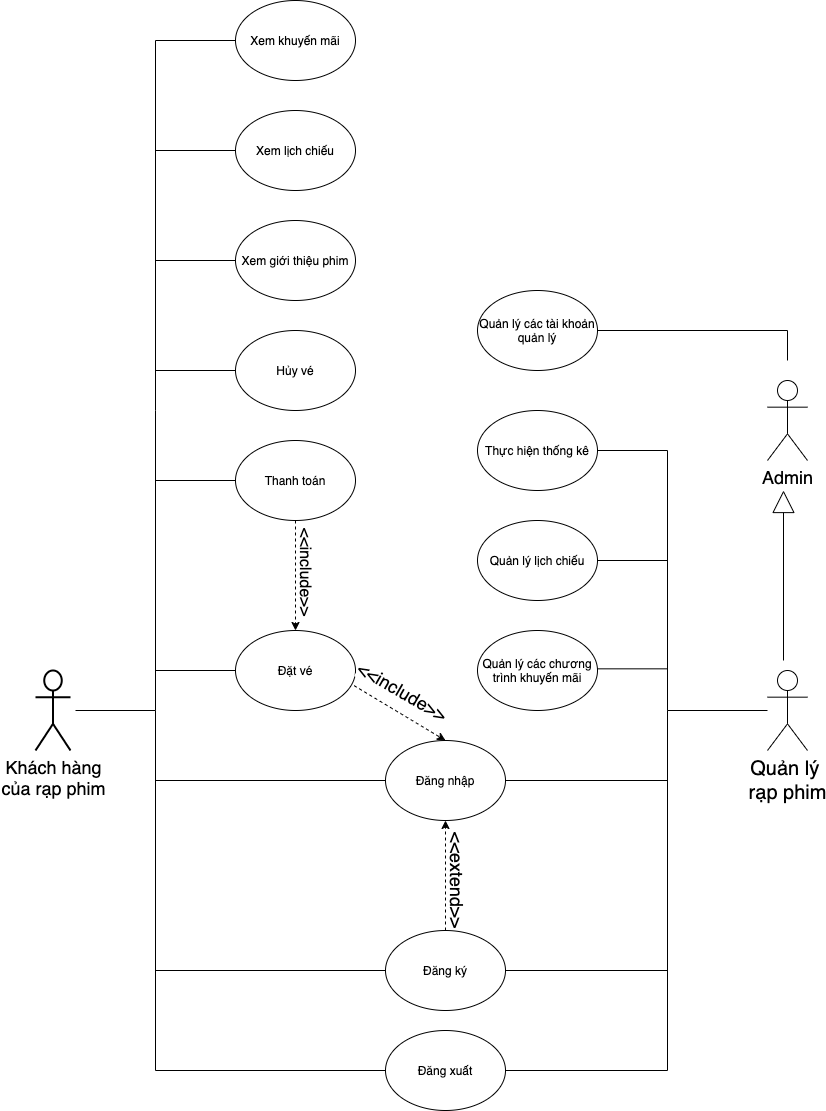
\includegraphics[scale = 0.6]{./UsecaseDiagram/usecase.png}
        \caption{Biểu đồ use case của hệ thống}
    \end{figure}

    \subsubsection{Ma trận truy xuất nguồn gốc}
    \begin{figure}[H]
        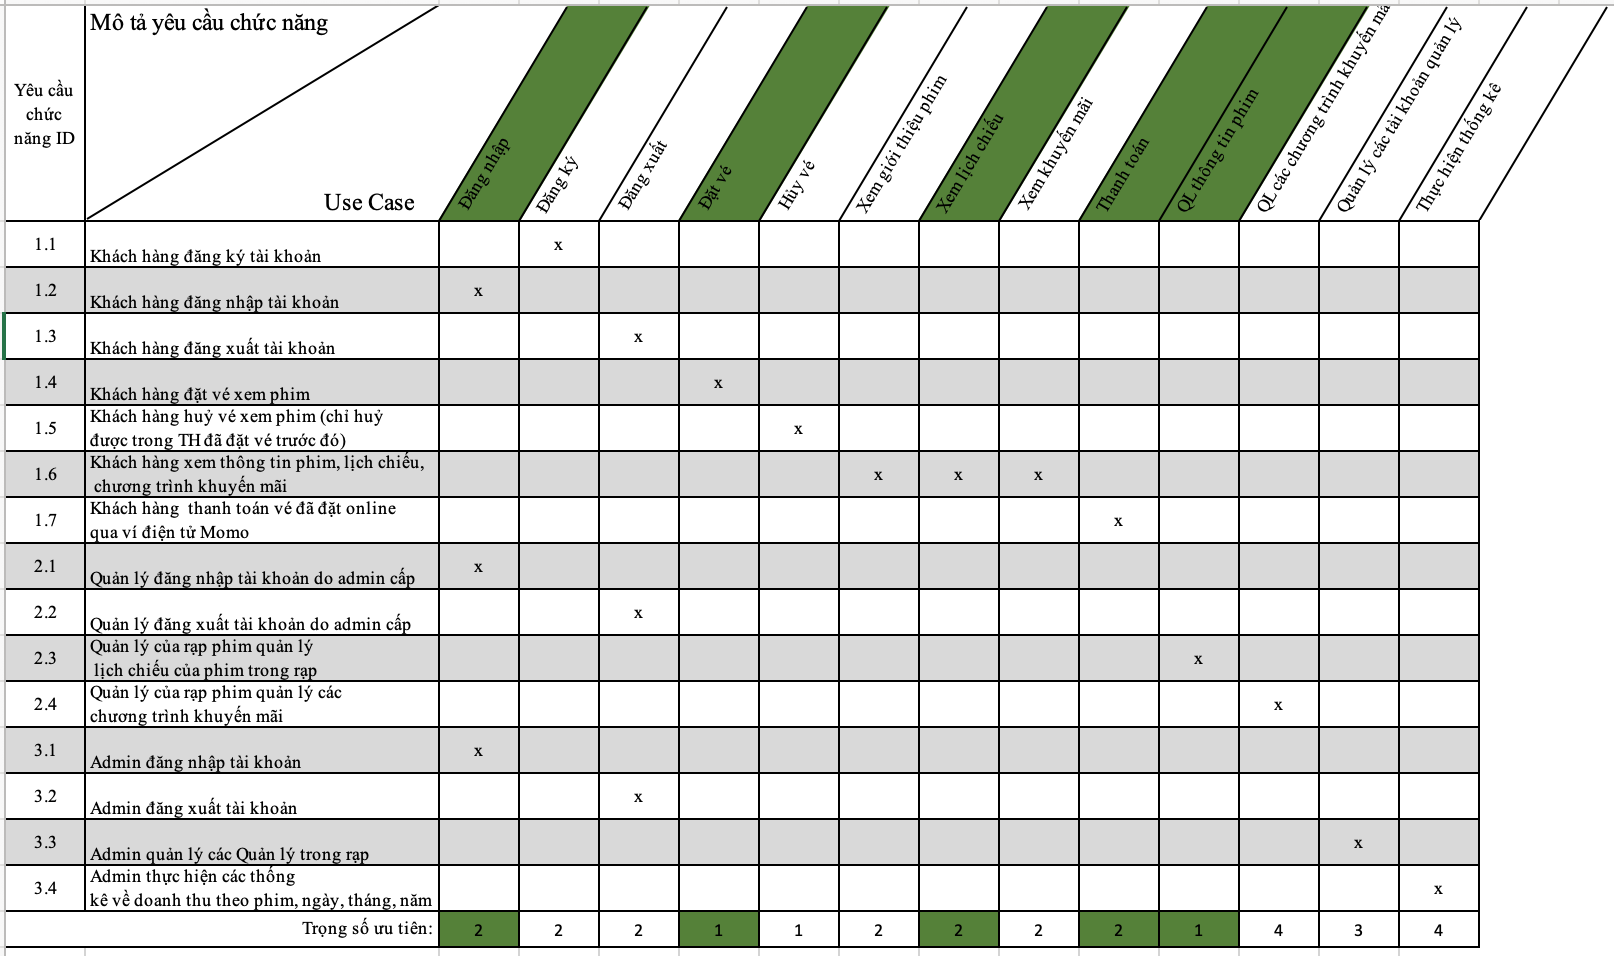
\includegraphics[angle=90,scale = 0.8]{TraceMatrix/traceMatrix.png}
        \caption{Ma trận truy xuất nguồn gốc}
    \end{figure}

    \subsubsection{Đặc tả use case}
    \begin{itemize}
        \item Use case Đăng nhập
        \begin{table}[H]
            \begin{tabular}{|l|l|}
            \hline
            ID                   & 1                                                                        \\ \hline
            Tên use case         & Đăng nhập                                                                \\ \hline
            Tóm tắt              & \begin{tabular}[c]{@{}l@{}}Giúp \textit{khách hàng của rạp, quản lý của rạp, admin} đăng nhập vào\\ hệ thống \end{tabular}\\ \hline
            Tác nhân             & Khách hàng của rạp, quản lý của rạp, admin                               \\ \hline
            Điều kiện tiên quyết & Thông tin về các tài khoản đã được lưu trong database                    \\ \hline
            Kết quả              & Khách hàng của rạp, quản lý của rạp, admin đăng nhập thành công          \\ \hline
            Kịch bản chính &\begin{tabular}[c]{@{}l@{}}1. Actor chọn chức năng Đăng nhập\\ 2. Hệ thống sẽ hiển thị trang đăng nhập\\3. Actor nhập tài khoản và nhấn đăng nhập\\4. Hệ thống kiểm tra tài khoản của Actor\\5. Hệ thống thông báo đăng nhập thành công \end{tabular} \\ \hline
            Kịch bản phụ &\begin{tabular}[c]{@{}l@{}}Tại bước 2, nếu khách hàng của rạp chưa có tài khoản\\   - 2.1. Khách hàng của rạp chọn chức năng Đăng ký \\   - 2.2. Hệ thống chuyển sang trang Đăng ký\\ Tại bước 4, nếu thông tin tài khoản sai hoặc không tồn tại, hệ thống \\sẽ báo lỗi tài khoản\end{tabular} \\ \hline
            Ràng buộc phi chức năng &\begin{tabular}[c]{@{}l@{}}Hệ thống đã lưu thông tin đã được mã hoá về tài khoản, mật khẩu \\của người dùng trong database\\Thời gian phản hồi của hệ thống dưới 1s \end{tabular}\\ \hline
            \end{tabular}
            \caption{Bảng đặc tả use case Đăng nhập}
        \end{table}

        \item Use case Đặt vé
        \begin{table}[H]
            \begin{tabular}{|l|l|}
            \hline
            ID                      & 4                                        \\ \hline
            Tên use case            & Đặt vé                                   \\ \hline
            Tóm tắt                 & Giúp \textit{khách hàng của rạp} có thể đặt vé xem phim \\ \hline
            Tác nhân                & Khách hàng của rạp                       \\ \hline
            Điều kiện tiên quyết &\begin{tabular}[c]{@{}l@{}}Trên hệ thống đã được thêm lịch chiếu của các phim\\ Khách hàng đã đăng nhập vào hệ thống\end{tabular} \\ \hline
            Kết quả                 & Chuyển sang bước checkout                \\ \hline
            Kịch bản chính &\begin{tabular}[c]{@{}l@{}}1. Khách hàng chọn phim muốn xem\\ 2. Khách hàng nhấn vào nút “Đặt vé”\\ 3. Hệ thống sẽ hiển thị form đặt vé\\ 4. \textit{Khách hàng của rạp} chọn lịch chiếu, ghế và nhấn nút “Thanh toán”\\ 5. Hệ thống sẽ chuyển đến trang thanh toán online\end{tabular} \\ \hline
            Kịch bản phụ &\begin{tabular}[c]{@{}l@{}}Trong trường hợp khách hàng chưa đăng nhập:\\ - 0.1. Hệ thống thông báo “Vui lòng đăng nhập”\\ - 0.2. Hệ thống hiển thị trang đăng nhập\\ - 0.3. Khách hàng tiến hành đăng nhập vào hệ thống\\ Trong trường hợp không nhấn nút "Thanh toán" hoặc không thanh \\toán thì vé sẽ không được đặt\end{tabular} \\ \hline
            Ràng buộc phi chức năng & Thời gian phản hồi của hệ thống dưới 1s  \\ \hline
            \end{tabular}
            \caption{Bảng đặc tả use case Đặt vé}
        \end{table}

        \item Use case Xem thông tin phim
        \begin{table}[H]
            \begin{tabular}{|l|l|}
            \hline
            ID                      & 7                                                     \\ \hline
            Tên use case            & Xem thông tin về phim                                 \\ \hline
            Tóm tắt &\begin{tabular}[c]{@{}l@{}}Giúp \textit{khách hàng của rạp} xem được lịch chiếu và các thông tin khác \\của phim (trailer, mô tả phim)\end{tabular} \\ \hline
            Tác nhân                & Khách hàng của rạp                                    \\ \hline
            Điều kiện tiên quyết    & Bộ phim đã được quản lý thêm lịch chiếu trên hệ thống \\ \hline
            Kết quả                 & Thông tin về lịch chiếu ở các rạp                     \\ \hline
            Kịch bản chính &\begin{tabular}[c]{@{}l@{}}1. \textit{Khách hàng của rạp} nhấn nút “Xem lịch chiếu”\\ 2. Hệ thống hiển thị trang xem lịch chiếu\\ 3. \textit{khách hàng của rạp} chọn bộ phim muốn xem lịch chiếu\\ 4. Hệ thống hiển thị lịch chiếu và thông tin của phim (bao gồm\\ trailer, mô tả)\end{tabular} \\ \hline
            Kịch bản phụ            & \begin{tabular}[c]{@{}l@{}}ád\\ ád\end{tabular}       \\ \hline
            Ràng buộc phi chức năng & Thời gian phản hồi của hệ thống dưới 1s               \\ \hline
            \end{tabular}
            \caption{Bảng đặc tả use case Xem thông tin phim}
        \end{table}

        \item Use case Thanh toán online
        \begin{table}[H]
            \begin{tabular}{|l|l|}
            \hline
            ID                      & 9                                                                                       \\ \hline
            Tên use case            & Thanh toán online                                                                       \\ \hline
            Tóm tắt                 & Thanh toán online bằng Momo cho vé đã đặt của khách hàng                                \\ \hline
            Tác nhân                & Khách hàng của rạp                                                                      \\ \hline
            Điều kiện tiên quyết    & \begin{tabular}[c]{@{}l@{}}Khách hàng đã tiến hành chọn vé thành công\\\end{tabular} \\ \hline
            Kết quả                 & \begin{tabular}[c]{@{}l@{}}Thông báo thanh toán thành công\\\end{tabular}            \\ \hline
            Kịch bản chính &\begin{tabular}[c]{@{}l@{}}1. Khách hàng chọn nút “Thanh toán”\\ 2. Hệ thống hiển thị trang thanh toán\\ 3. Khách hàng điền mã giảm giá (nếu có nhấn nút kiểm tra)\\ 4. Hệ thống kiểm tra mã giảm giá\\ 5. Khách hàng chọn nút “Tiếp tục”\\ 6. Hệ thống hiển thị trang quét mã Momo\\ 7. Khách hàng quét mã và thanh toán qua Momo\\ 8. Hệ thống kiểm tra việc thanh toán\\ 9. Hệ thống thông báo “Thanh toán thành công”\end{tabular} \\ \hline
            Kịch bản phụ &\begin{tabular}[c]{@{}l@{}}Tại bước 4 trong trường hợp mã giảm giá không đúng\\ - 4.1. Hệ thống thông báo “Mã giảm giá không tồn tại”\\ - 4.2. Quay lại bước 3\\ Tại bước 8 trong trường hợp kiểm tra thanh toán xảy ra lỗi\\ - 8.1. Hệ thống thông báo “Thanh toán xảy ra lỗi vui lòng thanh\\ toán lại”\\ - 8.2. Quay lại bước 5\end{tabular} \\ \hline
            Ràng buộc phi chức năng & Thời gian phản hồi của hệ thống dưới 1s                                                 \\ \hline
            \end{tabular}
            \caption{Bảng đặc tả use case Thanh toán online}
        \end{table}

        \item Use case Quản lý thông tin phim
        \begin{table}[H]
            \begin{tabular}{|l|l|}
            \hline
            ID                      & 10                                                                               \\ \hline
            Tên use case            & Quản lý thông tin phim                                                           \\ \hline
            Tóm tắt                 & \begin{tabular}[c]{@{}l@{}}Giúp “Quản lý” cập nhật lịch chiếu, thông tin phim, trailer về \\phim lên hệ thống \end{tabular}\\ \hline
            Tác nhân                & Quản lý                                                                          \\ \hline
            Điều kiện tiên quyết    & Quản lý đã đăng nhập vào hệ thống với vai trò quản lý                            \\ \hline
            Kết quả                 & \begin{tabular}[c]{@{}l@{}}Lịch chiếu được cập nhật\\\end{tabular}             \\ \hline
            Kịch bản chính &\begin{tabular}[c]{@{}l@{}}1. Quản lý nhấn vào nút “Quản lý lịch chiếu”\\ 2. Hệ thống hiển thị trang quản lý lịch chiếu\\ 3. Quản lý chỉnh sửa lịch chiếu, thông tin phim, trailer\\ 4. Hệ thống thông báo “Chỉnh sửa thành công”\end{tabular} \\ \hline
            Kịch bản phụ &\begin{tabular}[c]{@{}l@{}}Tại bước 3 trong trường hợp chỉnh sửa lịch chiếu bị xung đột\\ - 3.1. Hệ thống hiển thị thông báo “Lịch phim bị trùng. Thao tác\\ thất bại”\\ - 3.2. Quay lại bước 2\end{tabular} \\ \hline
            Ràng buộc phi chức năng & Thời gian phản hồi của hệ thống dưới 1s                                          \\ \hline
            \end{tabular}
            \caption{Bảng đặc tả use case Quản lý thông tin phim}
        \end{table}
    \end{itemize}

    \subsection{Biểu đồ tuần tự}
    \begin{itemize}
        \item Use case Đăng nhập
        \begin{figure}[H]
            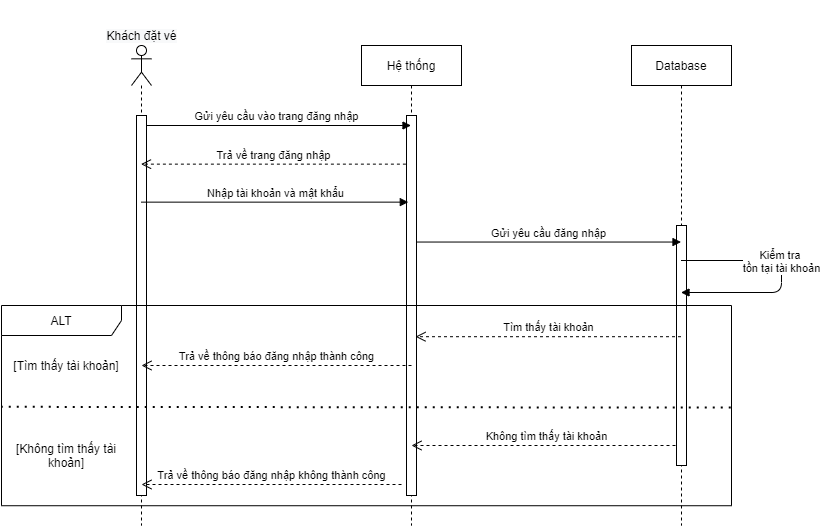
\includegraphics[scale = 0.65]{SequenceDiagram/Khách_Đăng nhập.png}
            \caption{Biểu đồ tuần tự của use case Đăng nhập}
        \end{figure}

        \item Use case Đặt vé
        \begin{figure}[H]
            \includegraphics[scale = 0.65]{SequenceDiagram/Đặt vé.png}
            \caption{Biểu đồ tuần tự của use case Đặt vé}
        \end{figure}
        
        \item Use case Xem thông tin phim
        \begin{figure}[H]
            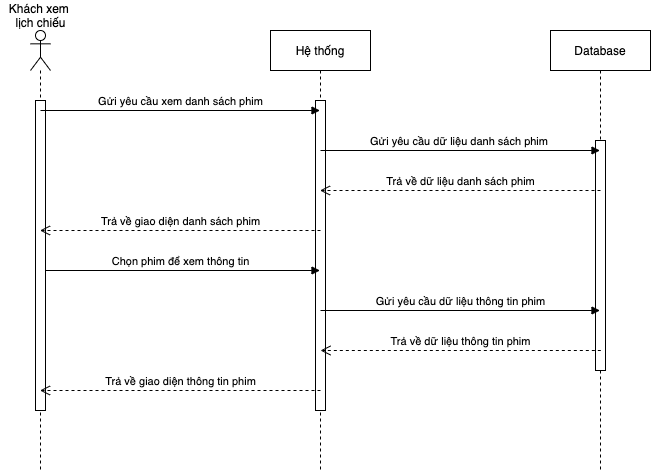
\includegraphics[scale = 0.7]{SequenceDiagram/Khách_Xem thông tin phim.png}
            \caption{Biểu đồ tuần tự của use case Xem thông tin phim}
        \end{figure}
        
        \item Use case Thanh toán online
        \begin{figure}[H]
            \includegraphics[scale = 0.7]{SequenceDiagram/Thanh toán.png}
            \caption{Biểu đồ tuần tự cho use case Thanh toán online}
        \end{figure}
        
        \item Use case Quản lý thông tin phim
        \begin{figure}[H]
            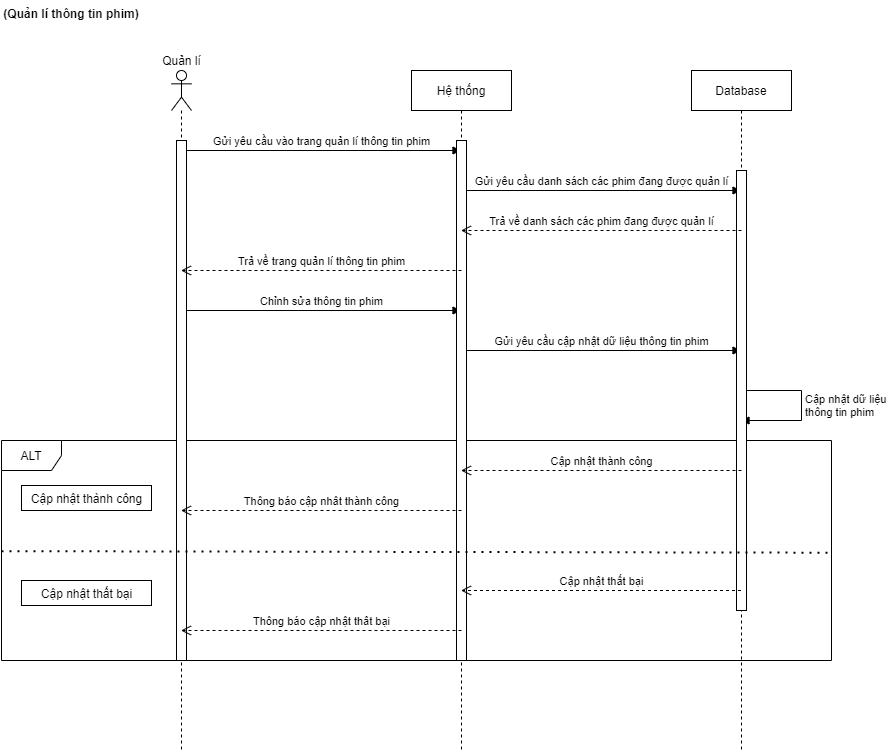
\includegraphics[scale = 0.65]{SequenceDiagram/Quản lí_Thông tin phim.png}
            \caption{Biểu đồ tuần tự của use case Quản lý thông tin phim}
        \end{figure}
    \end{itemize}
    \clearpage

    \section{Đặc tả giao diện người sử dụng}
    \label{sec:describeUI}

    \subsection{Thiết kế sơ bộ}
    \begin{enumerate}
        %Use case Đăng nhập
        \item Use case Đăng nhập
        \begin{figure}[H]
            \begin{center}
                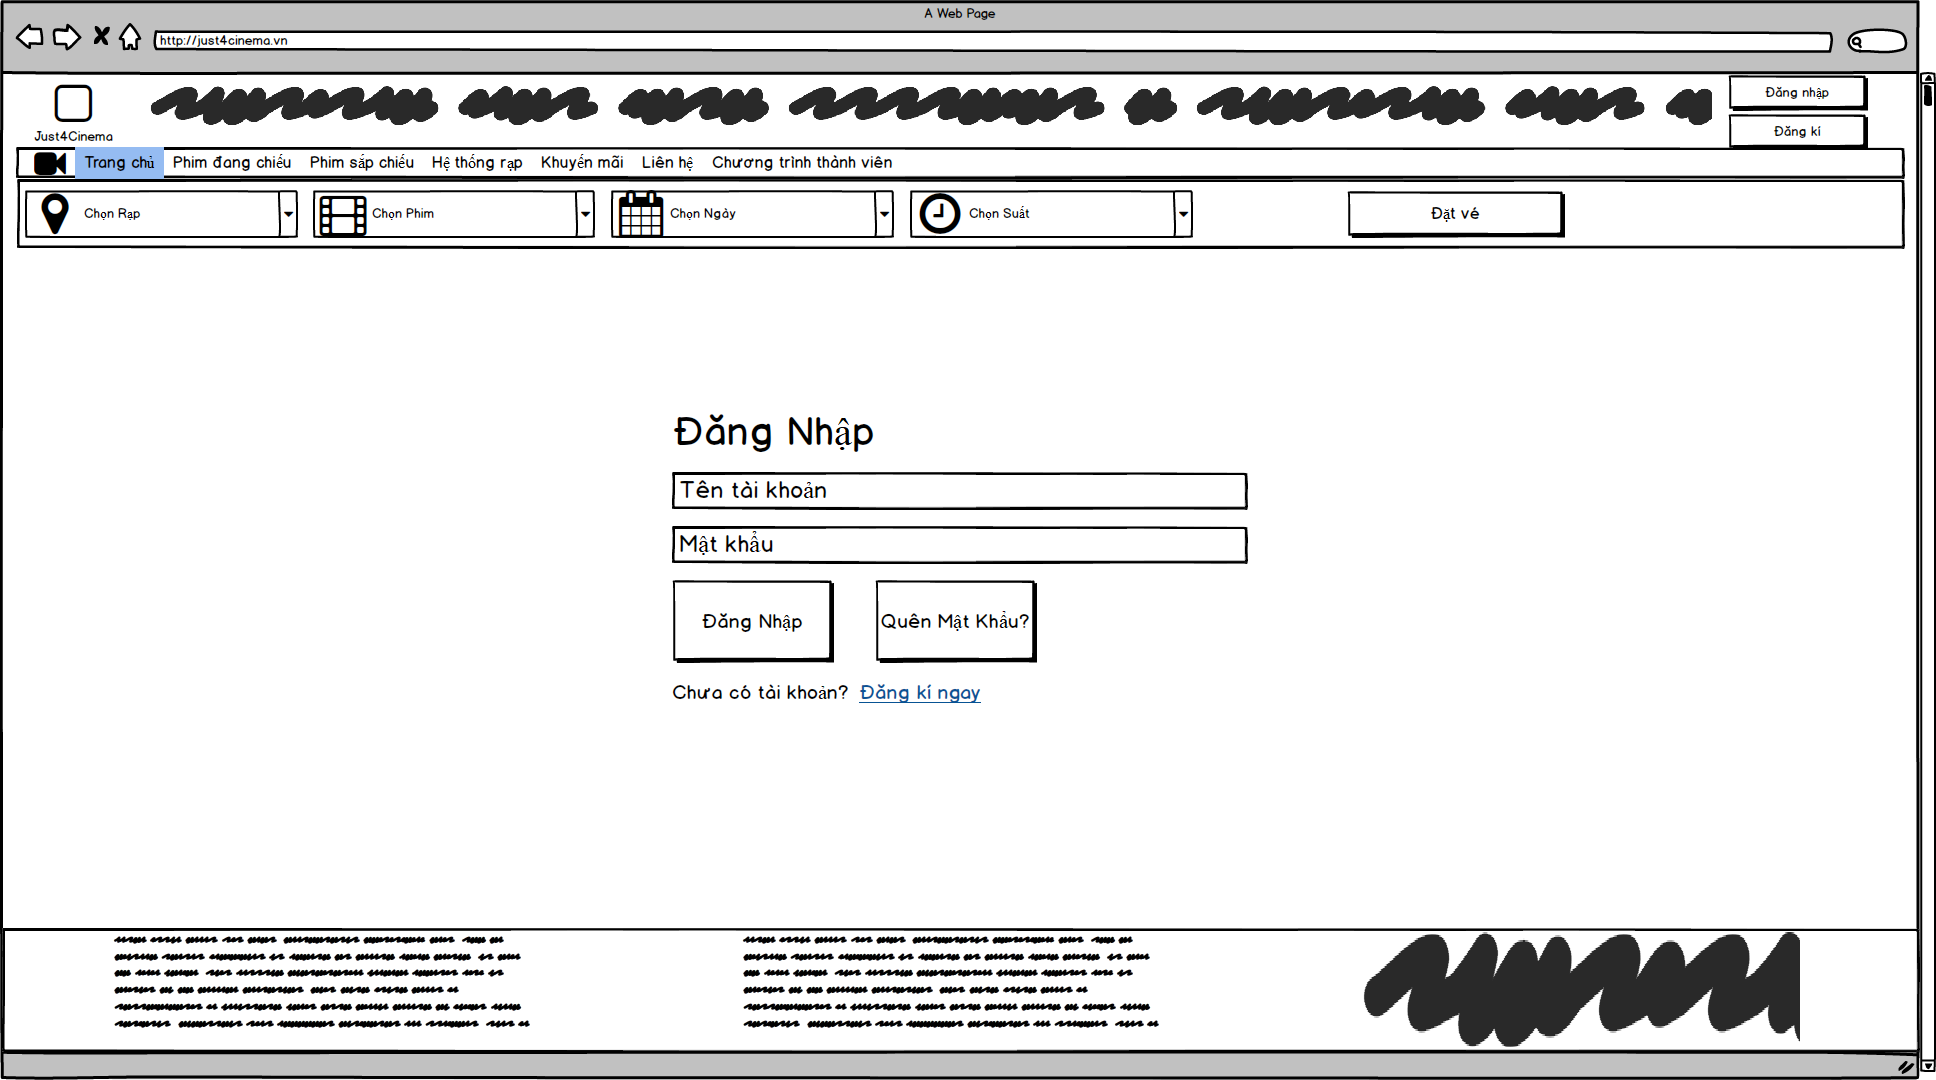
\includegraphics[scale = 0.25]{Wireframe/User/Đăng nhập.png}
                \caption{Giao diện đăng nhập của khách hàng rạp phim}
            \end{center}
        \end{figure}
        \begin{figure}[H]
            \begin{center}
                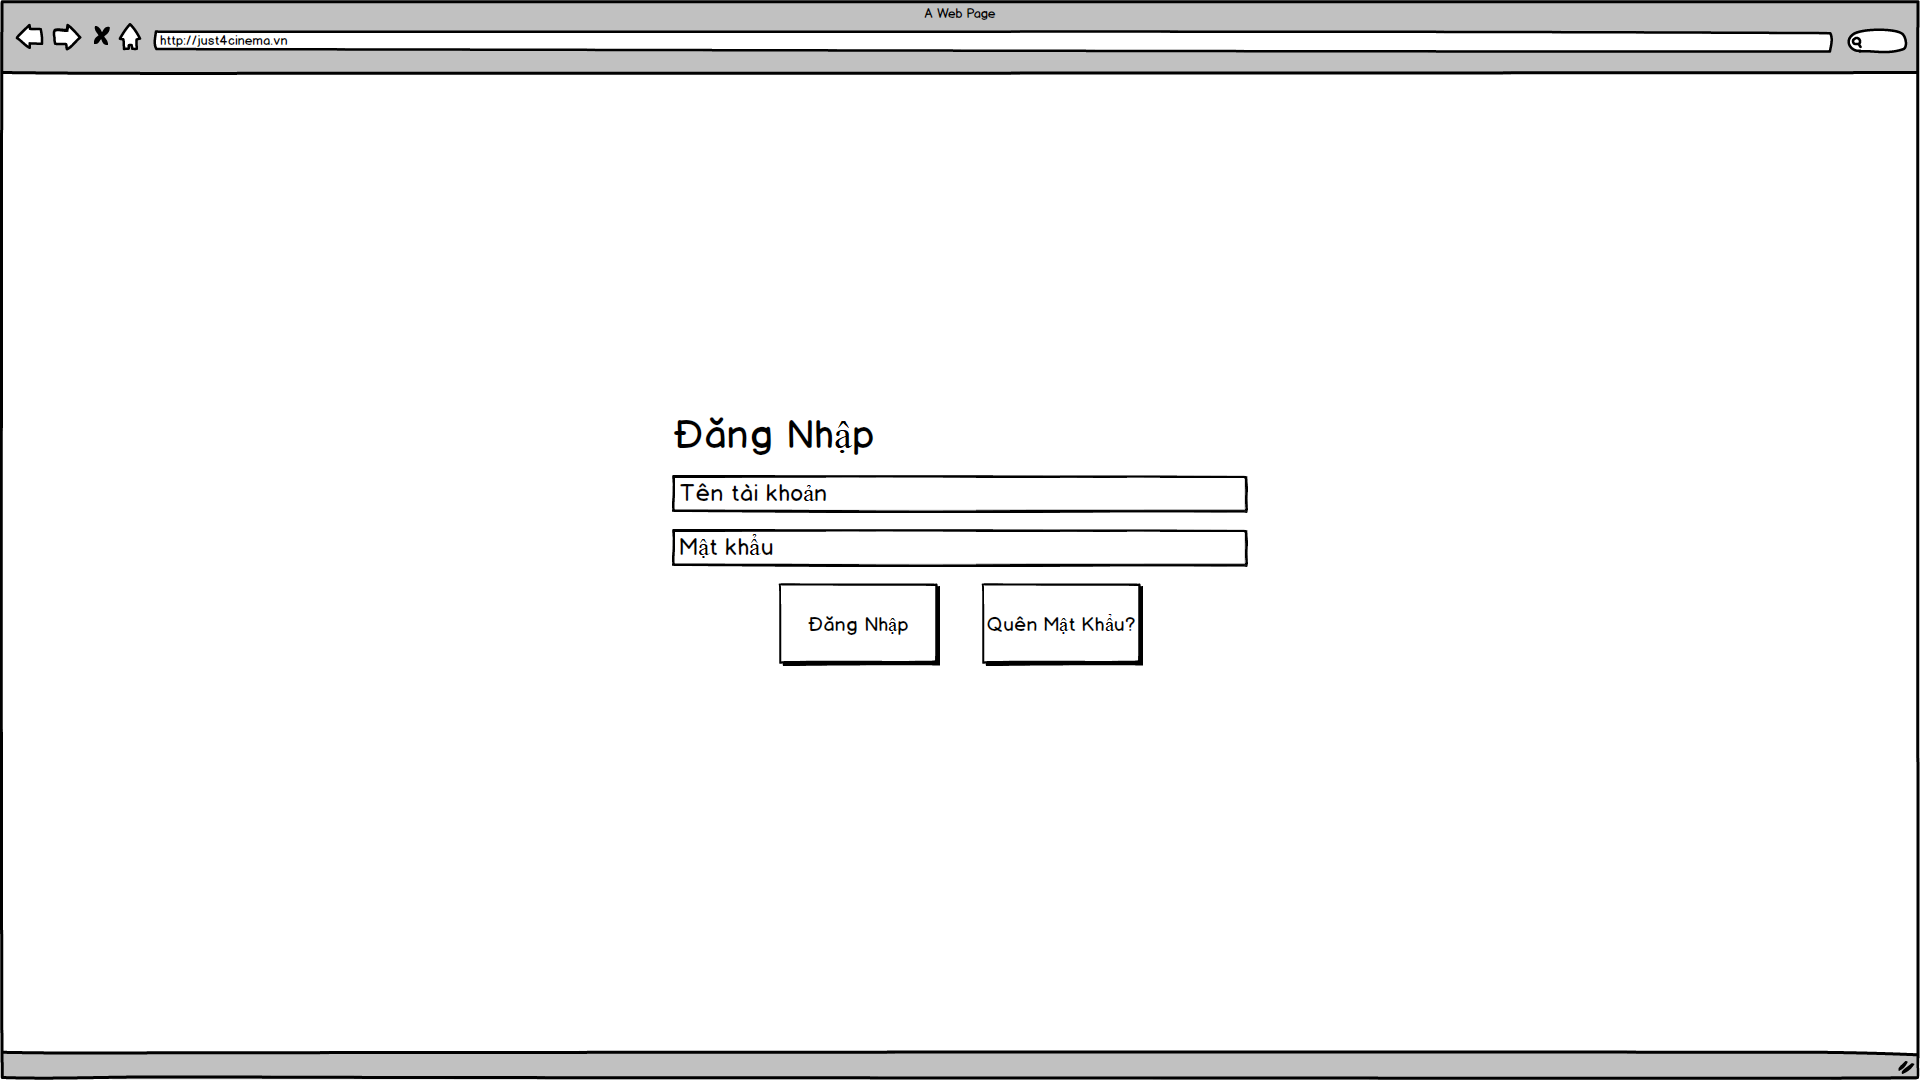
\includegraphics[scale = 0.25]{Wireframe/Manager/Quản lý_Đăng nhập.png}
                \caption{Giao diện đăng nhập của quản lý}
            \end{center}
        \end{figure}

        \begin{figure}[H]
            \begin{center}
                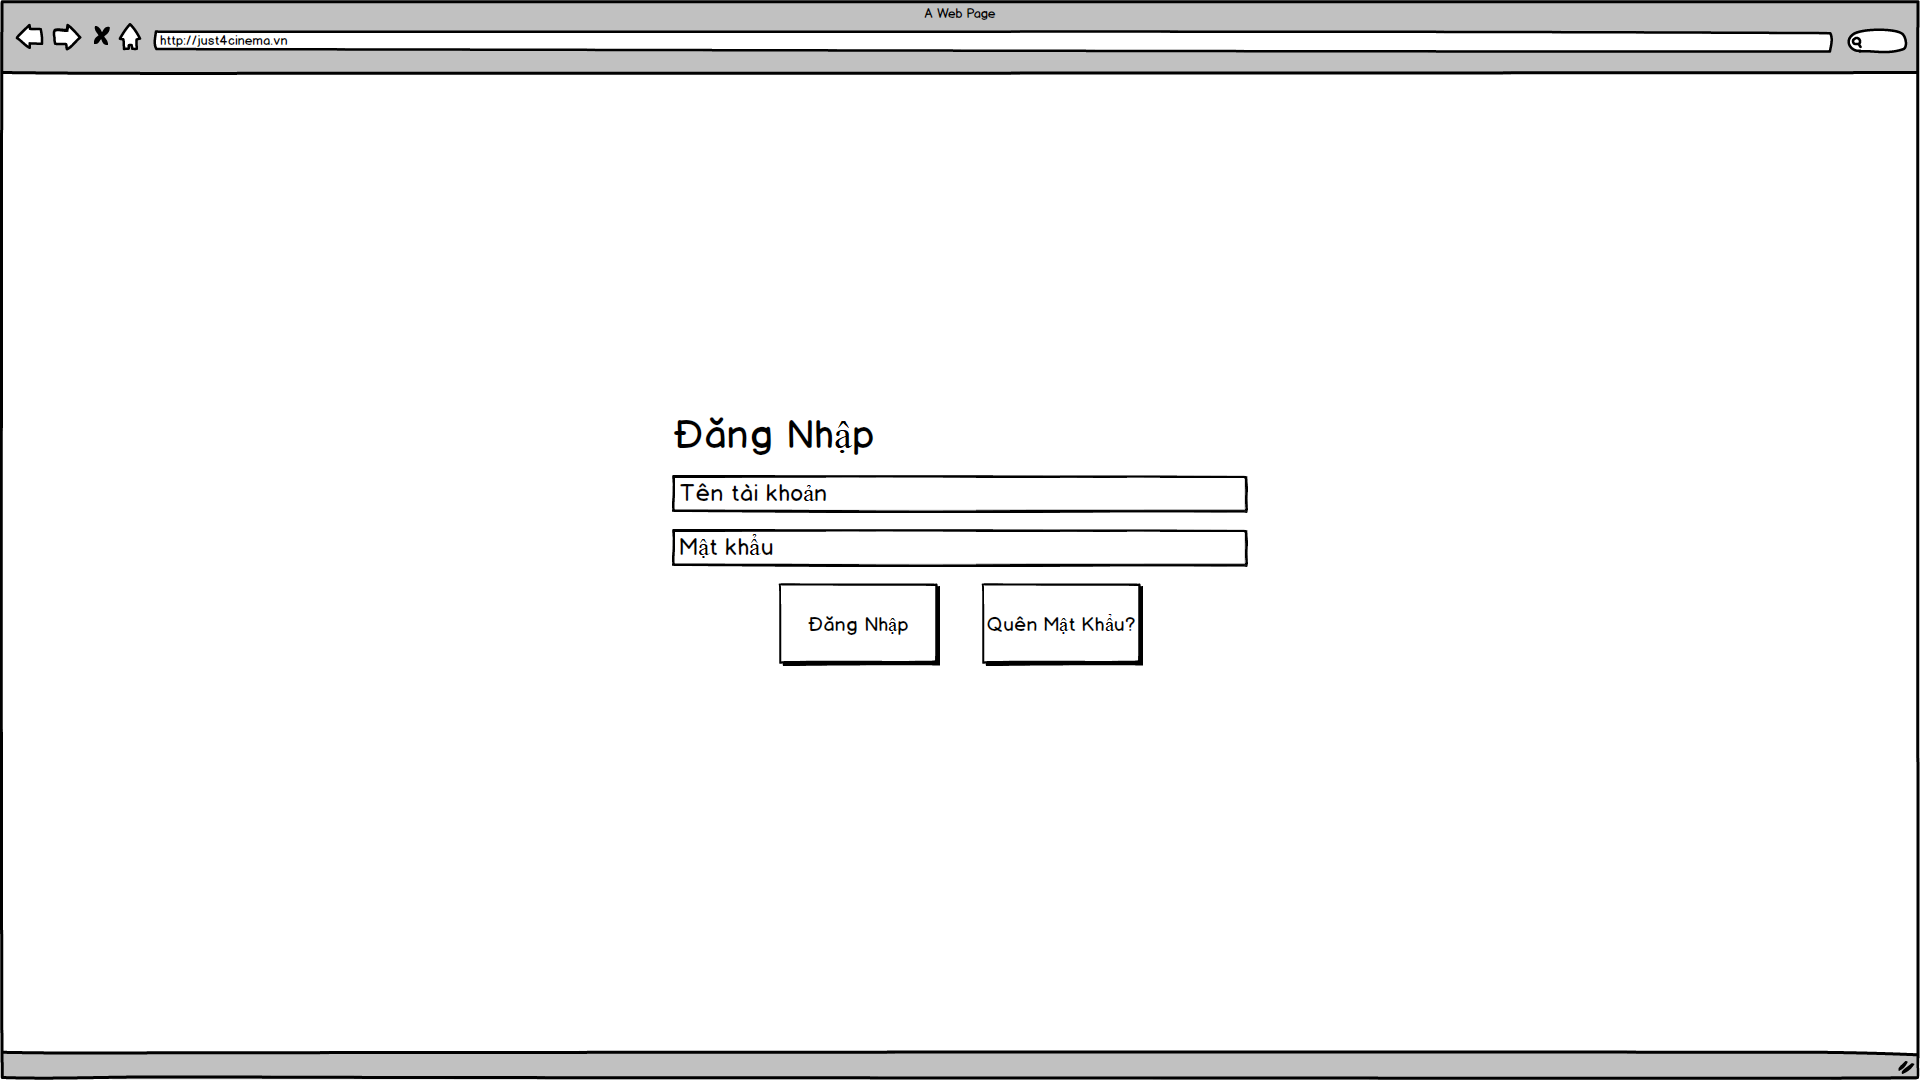
\includegraphics[scale = 0.25]{Wireframe/Admin/Admin_Đăng nhập.png}
                \caption{Giao diện đăng nhập của admin}
            \end{center}
        \end{figure}

        %Use case Đăng kí
        \item Use case Đăng kí
        \begin{figure}[H]
            \begin{center}
                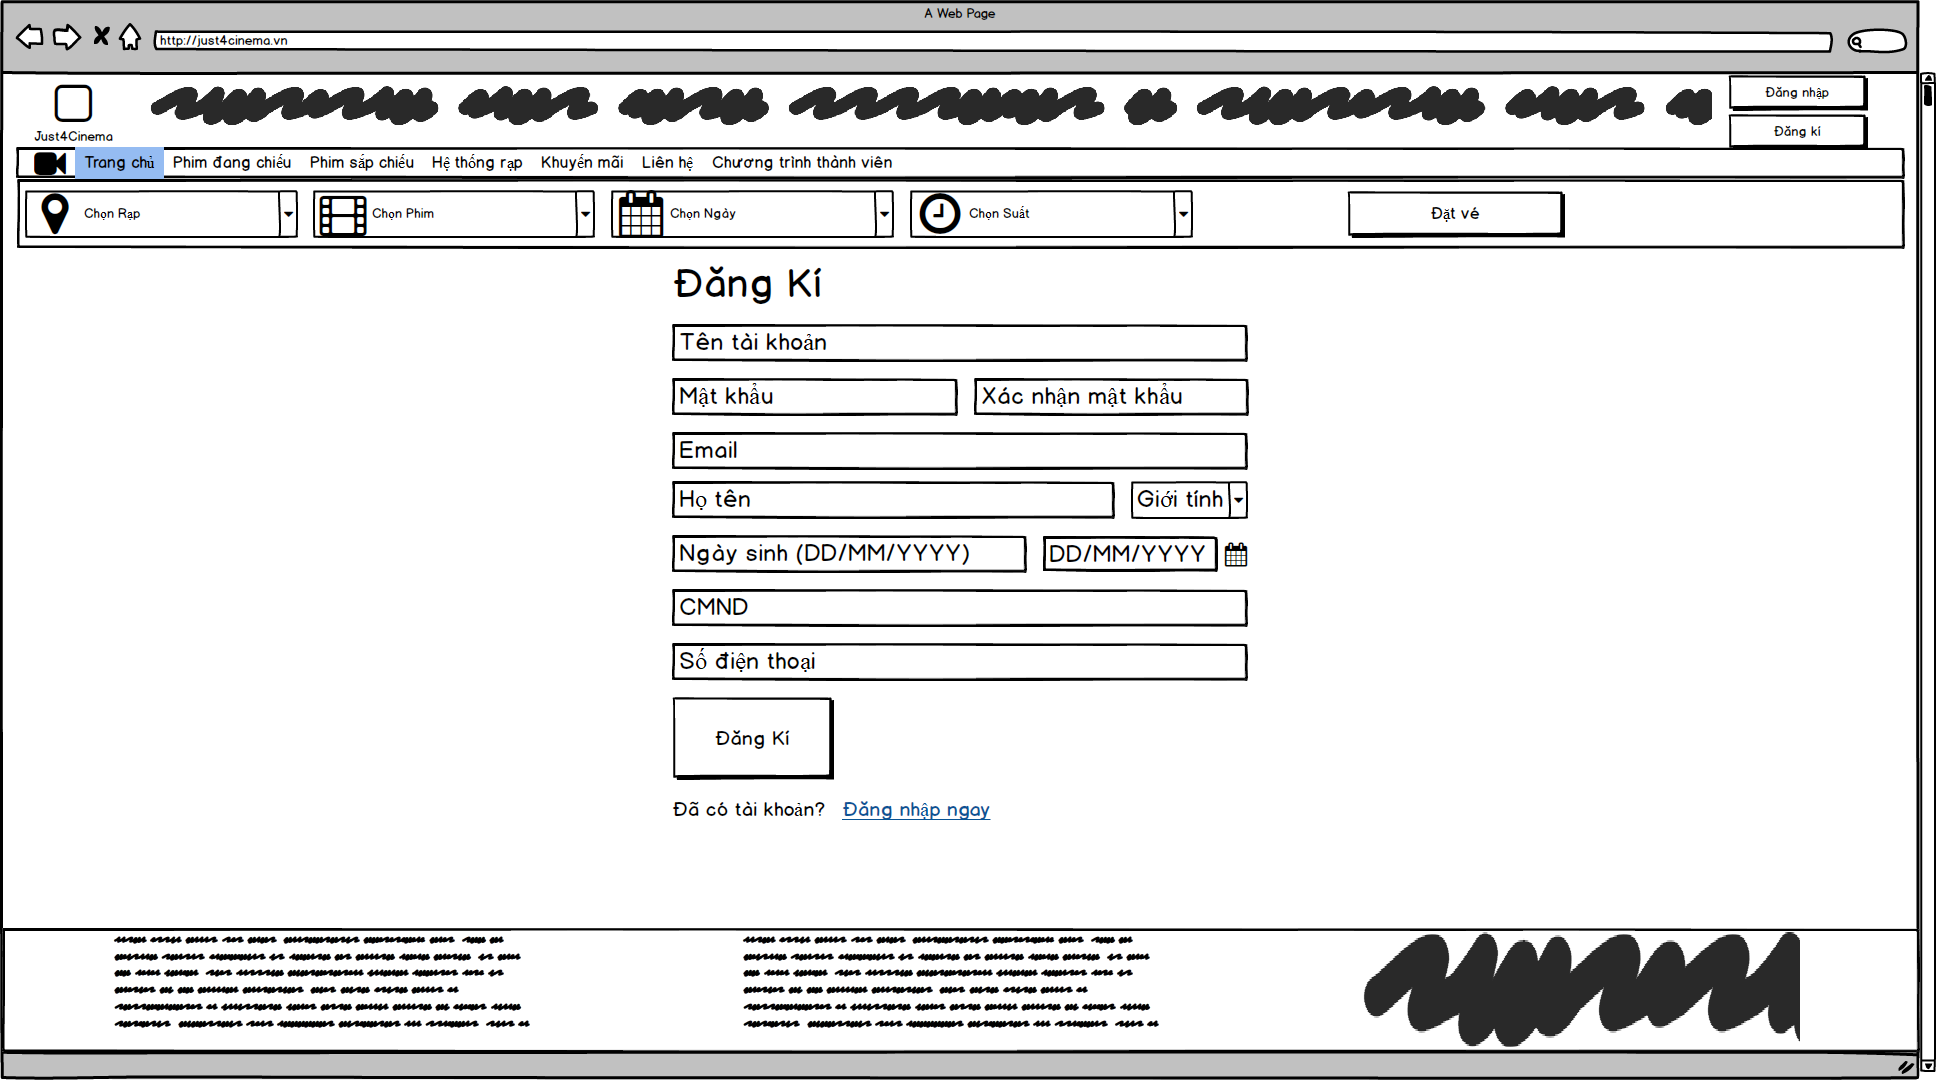
\includegraphics[scale = 0.25]{Wireframe/User/Đăng kí.png}
                \caption{Giao diện đăng kí của khách hàng rạp phim}
            \end{center}
        \end{figure}

        %Use case Đăng xuất
        \item Use case Đăng xuất
        \begin{figure}[H]
            \begin{center}
                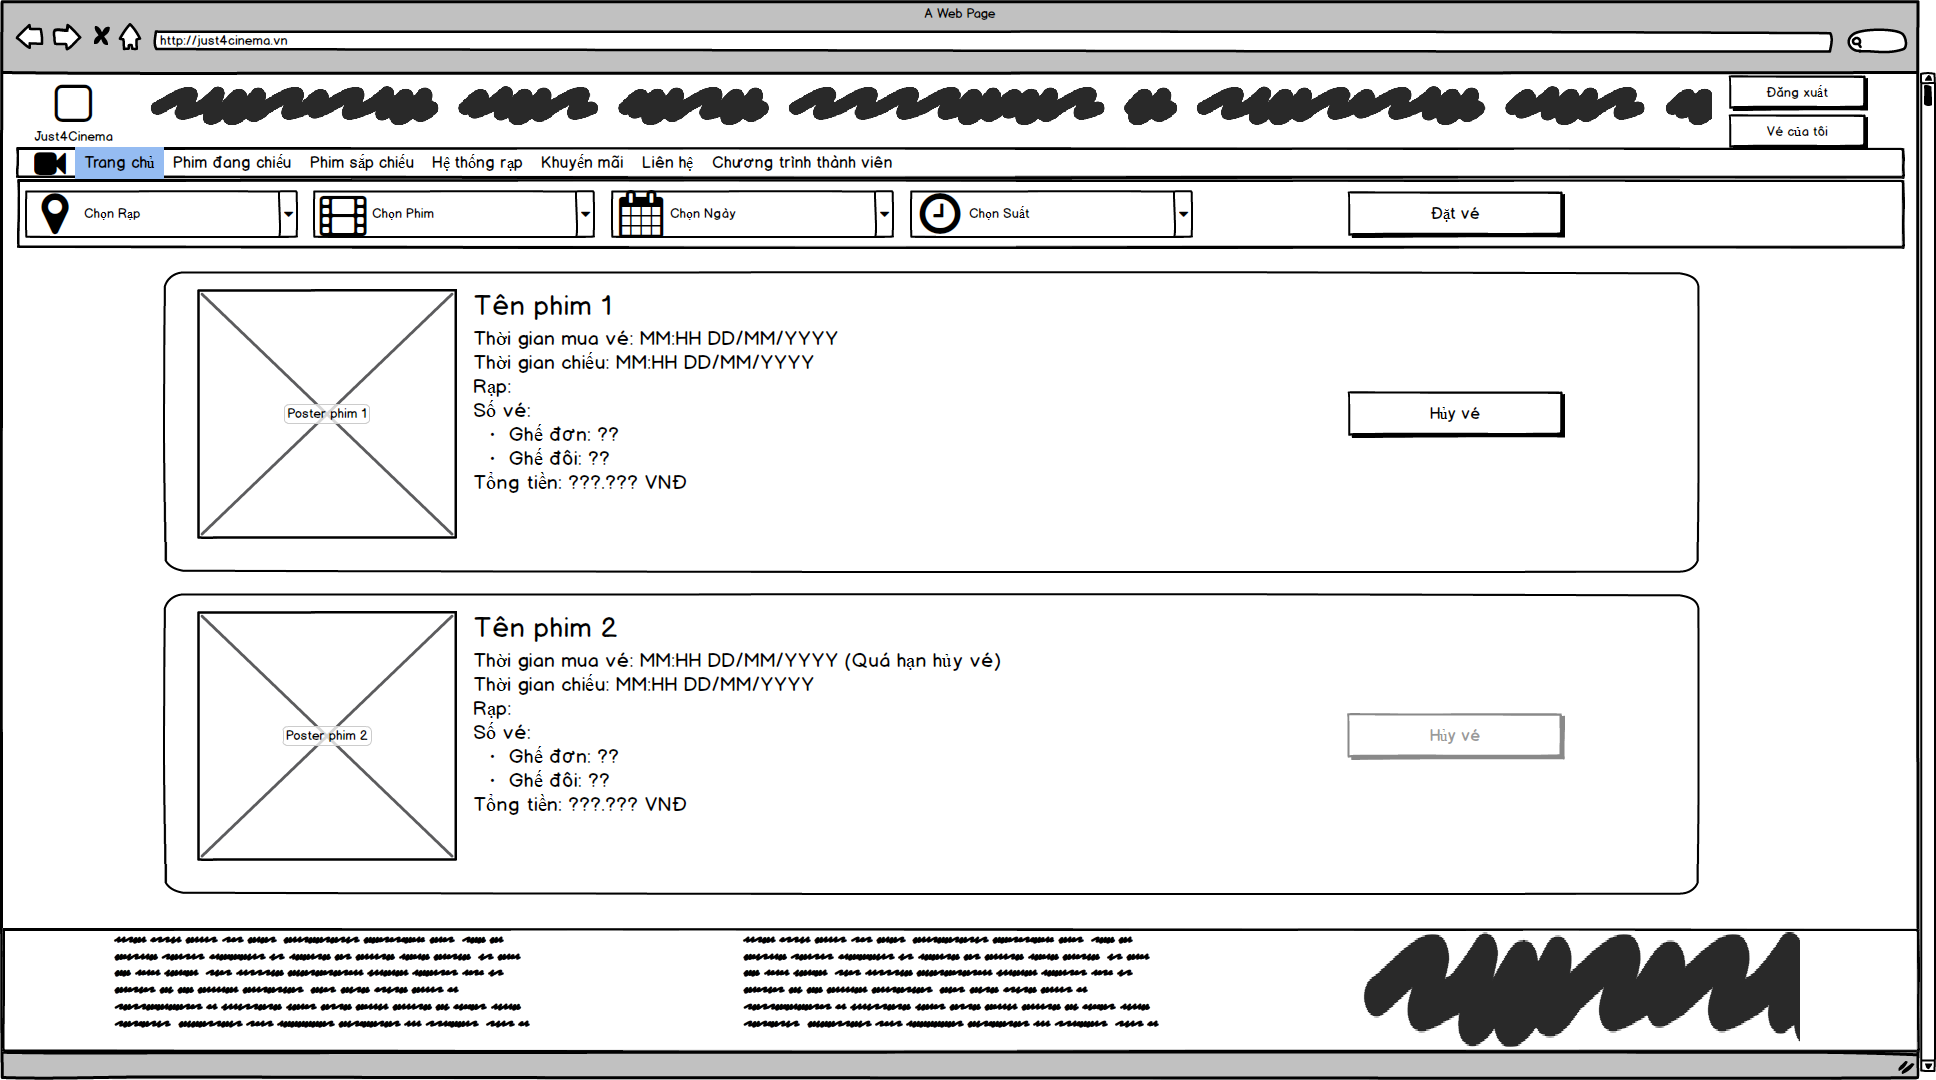
\includegraphics[scale = 0.25]{Wireframe/User/Vé của tôi.png}
                \caption{Nút Đăng xuất nằm tại góc phải màn hình của khách hàng của rạp}
            \end{center}
        \end{figure}
        \begin{figure}[H]
            \begin{center}
                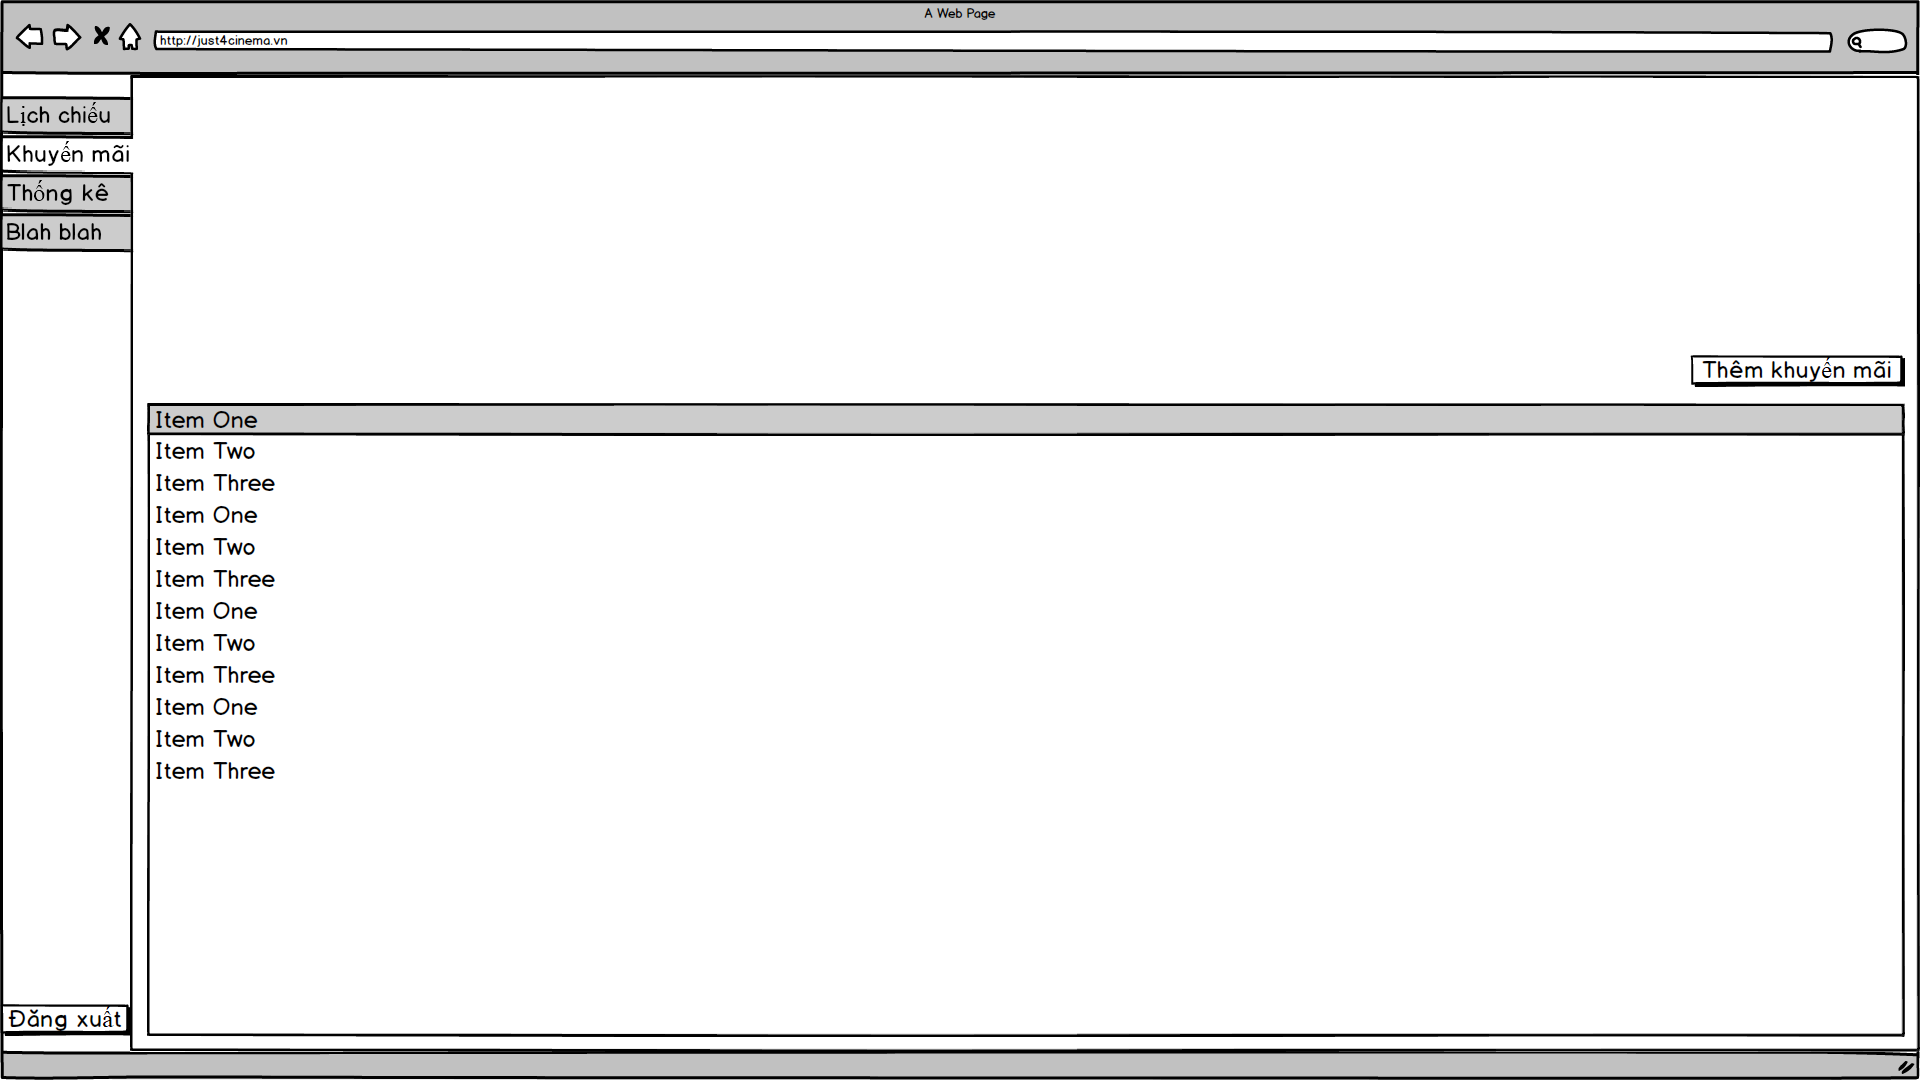
\includegraphics[scale = 0.25]{Wireframe/Manager/Quản lý_Dashboard_Khuyến mãi.png}
                \caption{Với quản lý: Nút đăng xuất sẽ nằm ở góc trái bên dưới sau khi đã đăng nhập}
            \end{center}
        \end{figure}
        \begin{figure}[H]
            \begin{center}
                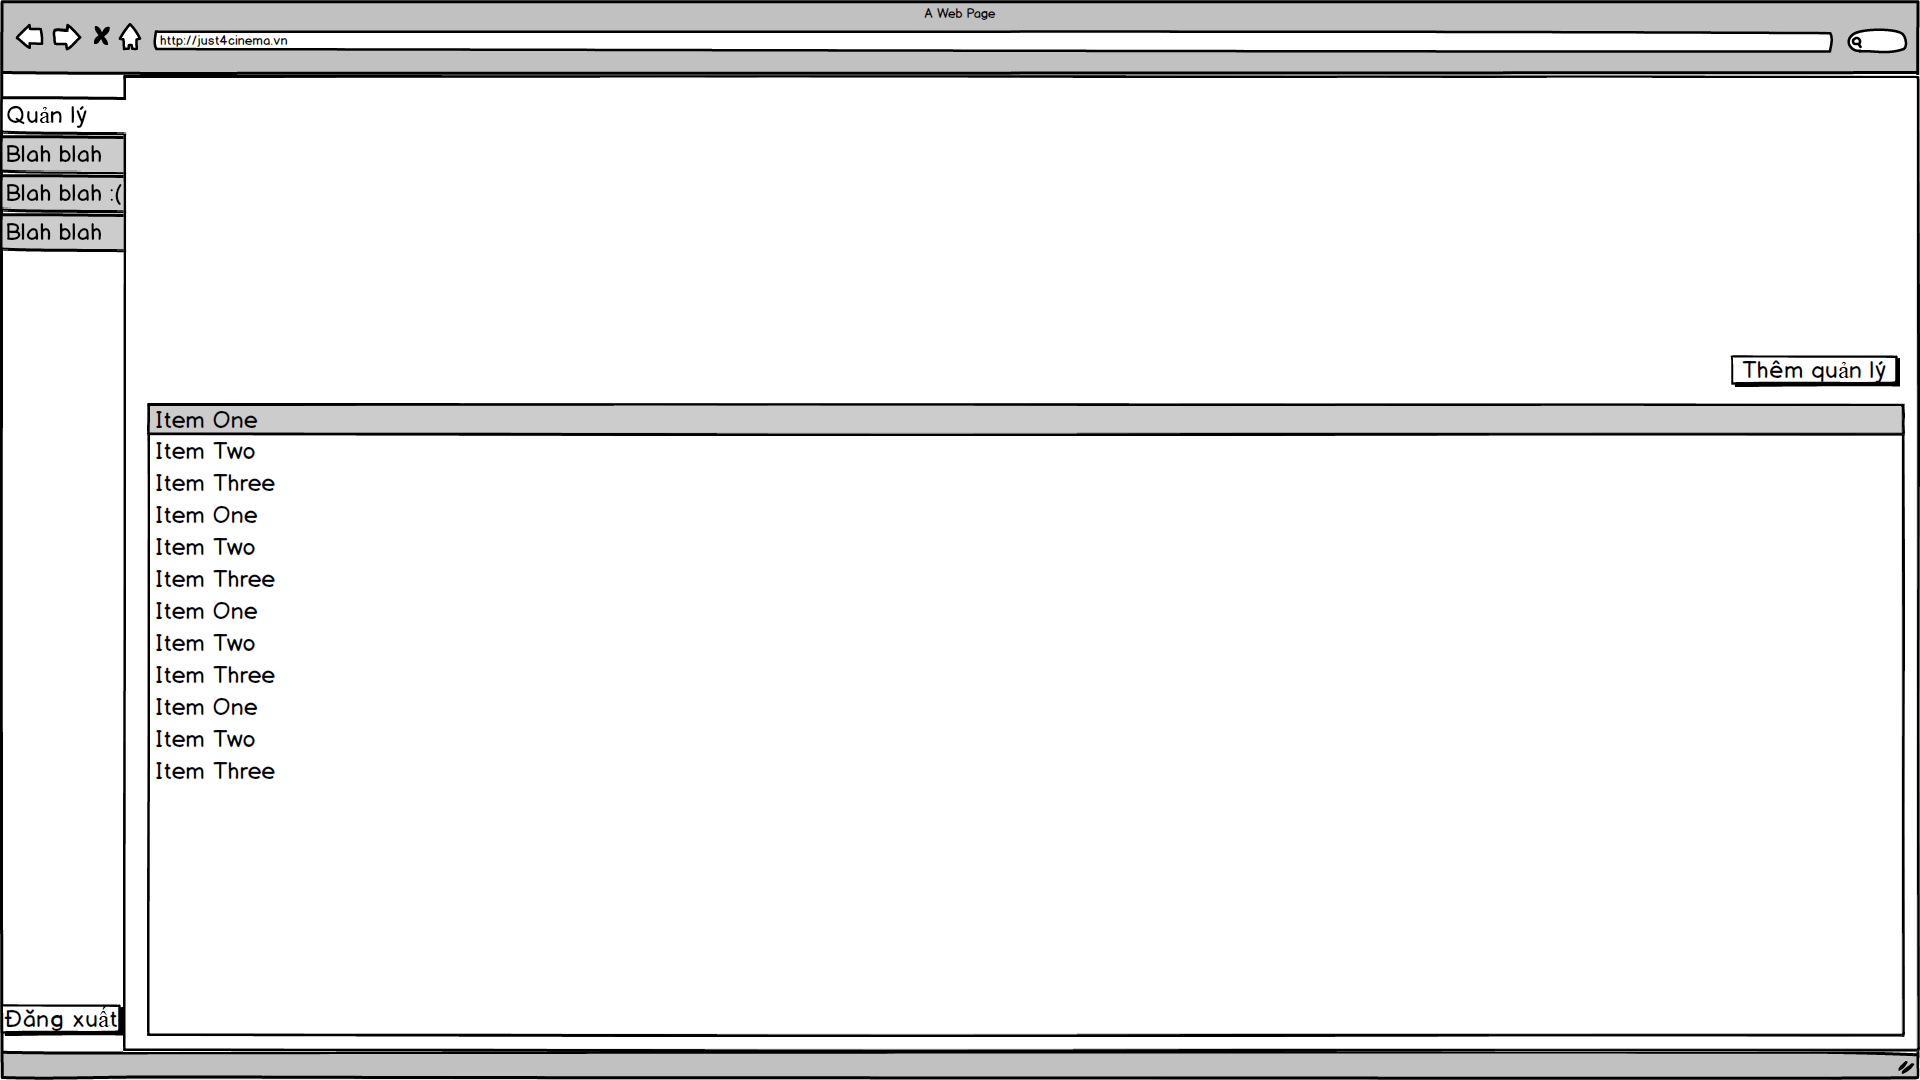
\includegraphics[scale = 0.25]{Wireframe/Admin/Admin_Quản lý.png}
                \caption{Với admin: Nút đăng xuất sẽ nằm ở góc trái bên dưới sau khi đã đăng nhập}
            \end{center}
        \end{figure}

        %Use case Đặt vé
        \item Use case Đặt vé
        \begin{figure}[H]
            \begin{center}
                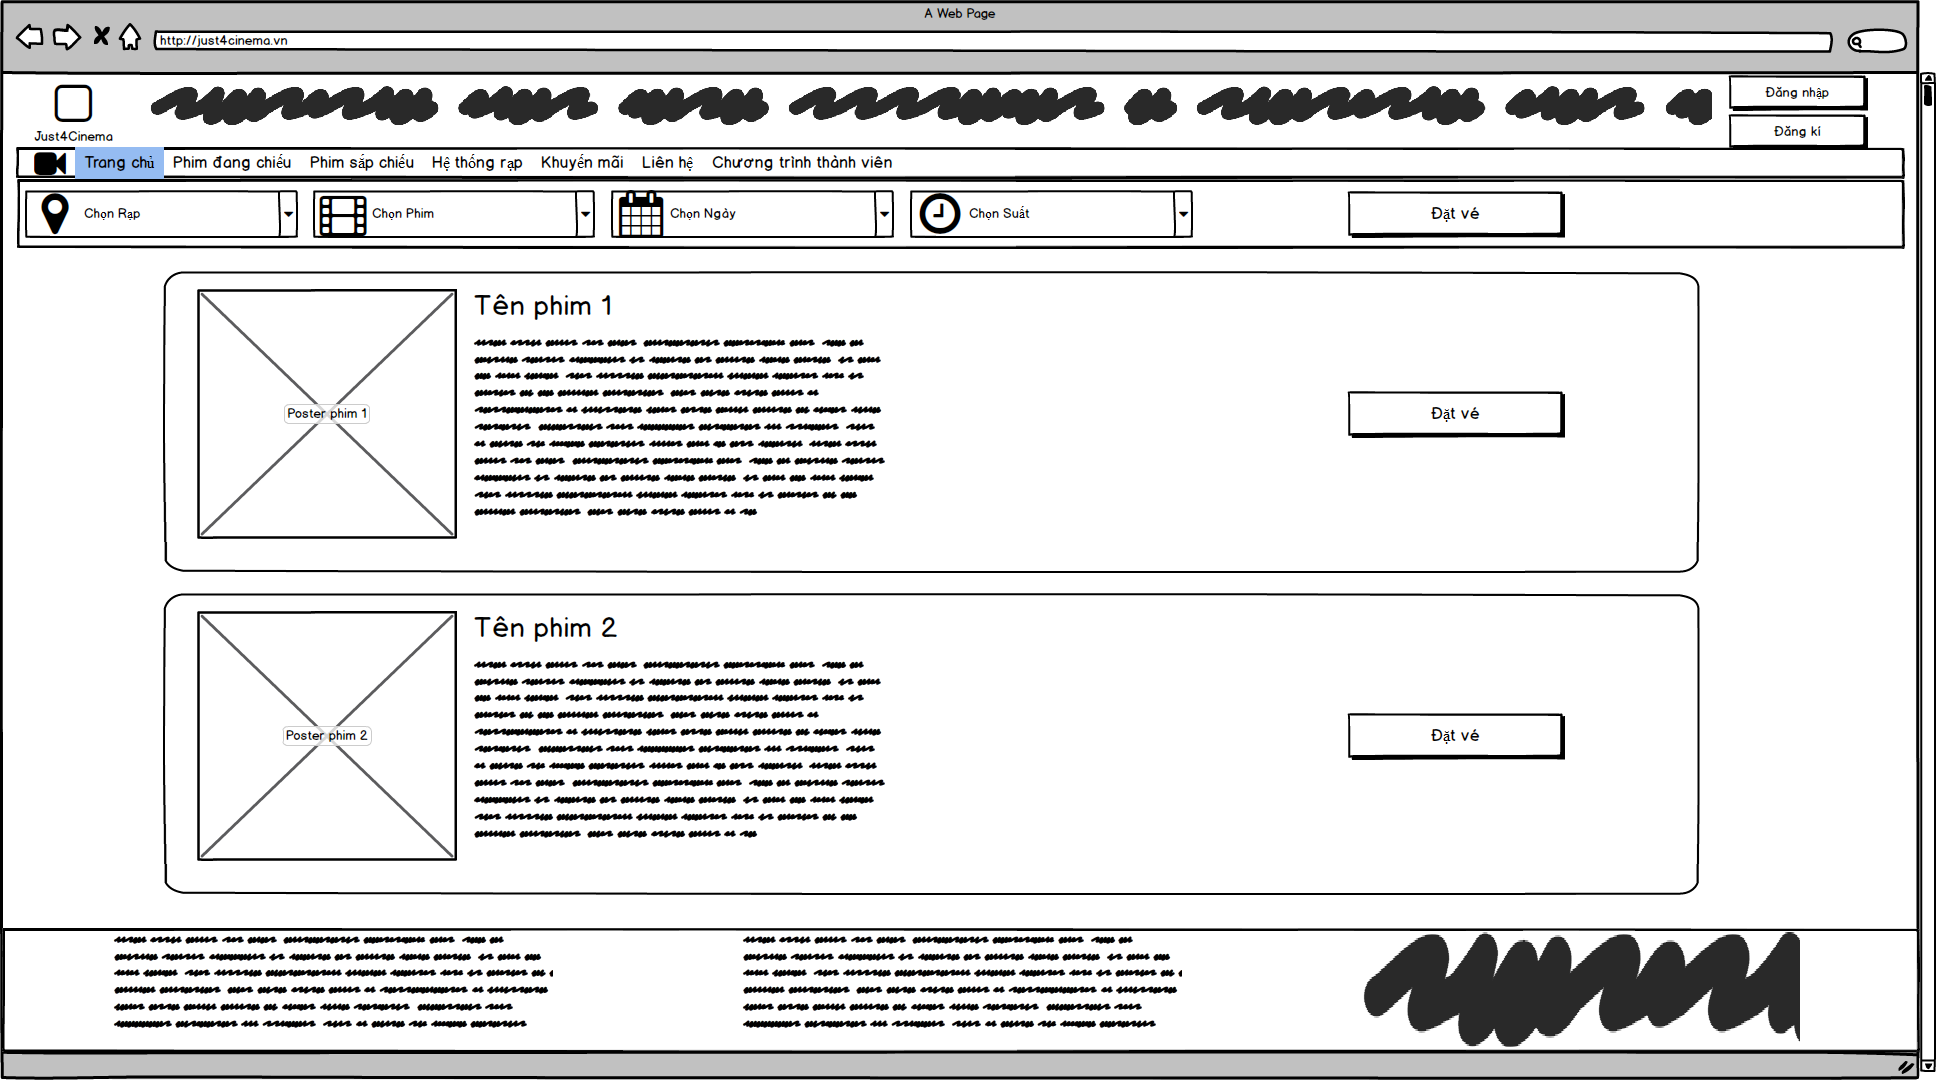
\includegraphics[scale = 0.25]{Wireframe/User/Phim đang chiếu_ Chọn phim.png}
                \caption{Giao diện xem phim đang chiếu}
            \end{center}
        \end{figure}

        \begin{figure}[H]
            \begin{center}
                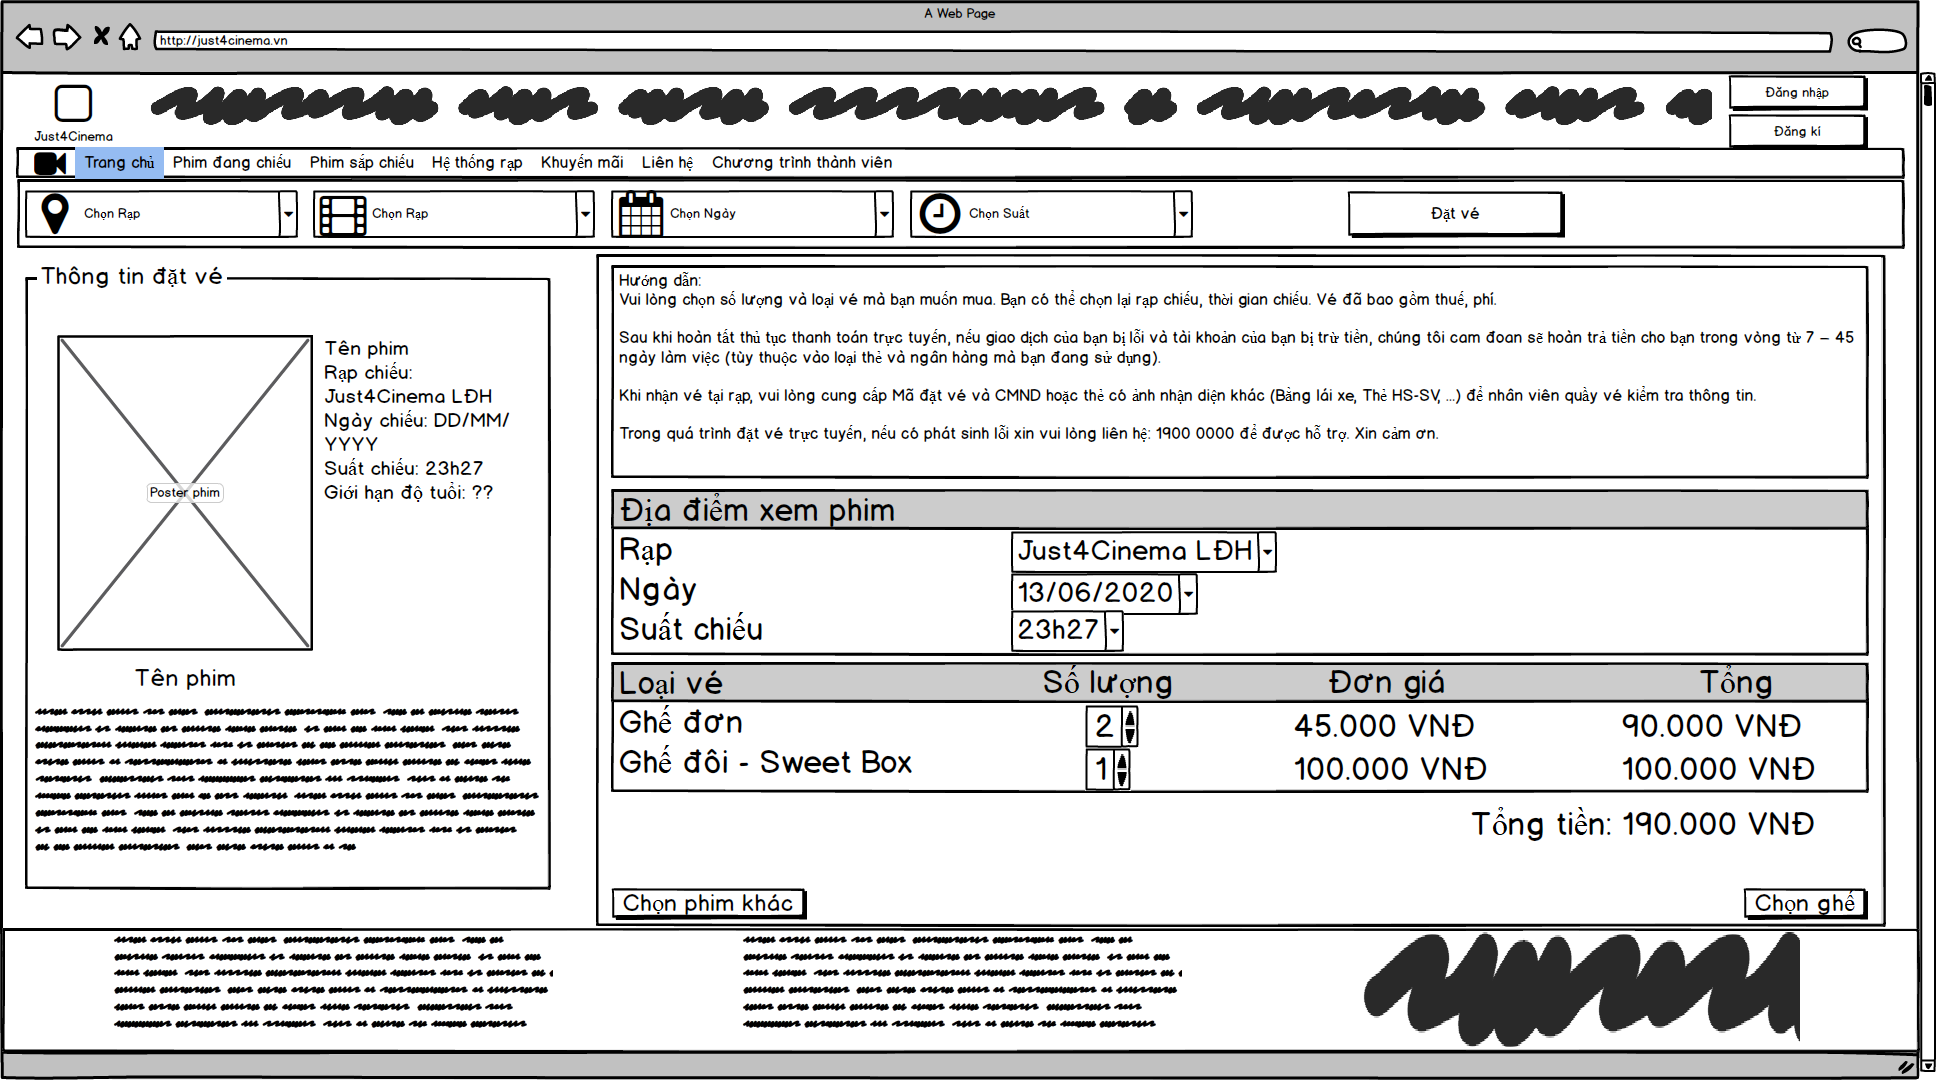
\includegraphics[scale = 0.25]{Wireframe/User/Đặt vé.png}
                \caption{Giao diện đặt vé của khách hàng rạp phim}
            \end{center}
        \end{figure}

        \begin{figure}[H]
            \begin{center}
                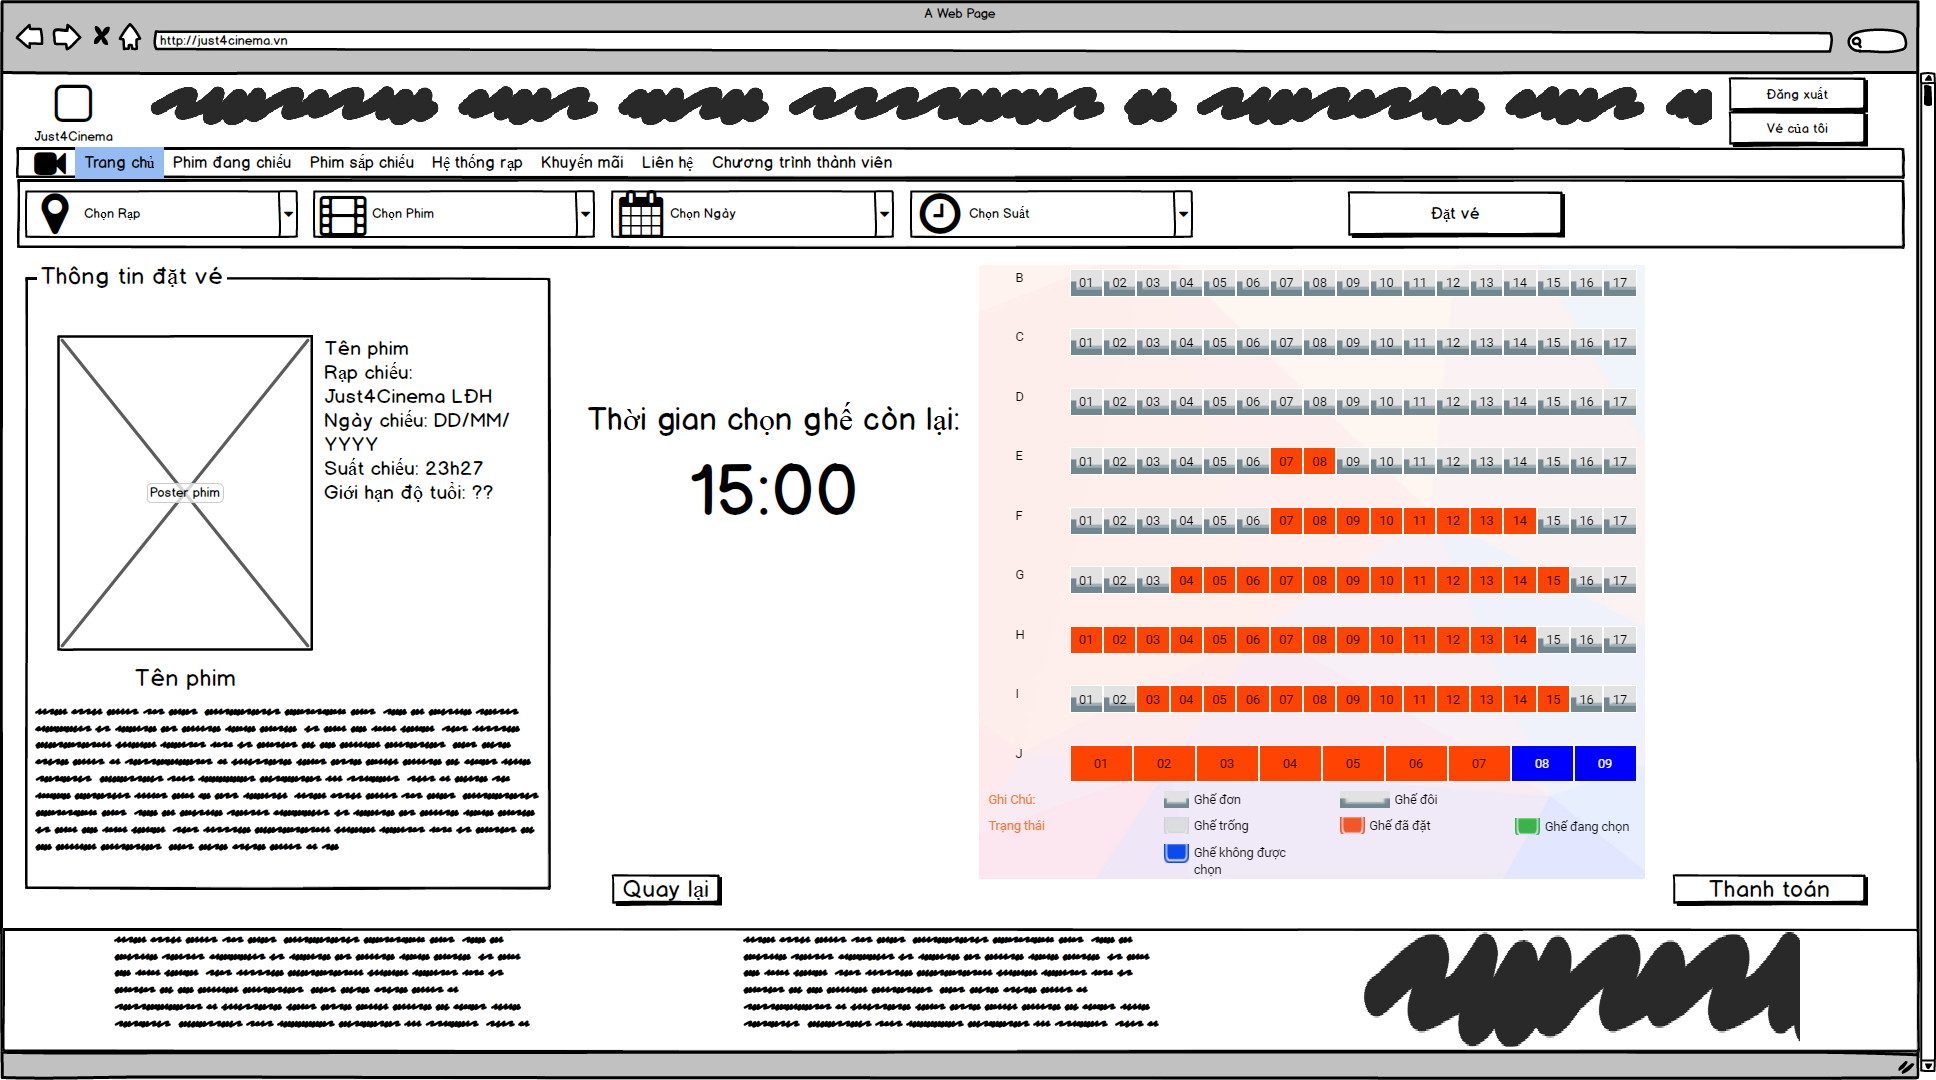
\includegraphics[scale = 0.25]{Wireframe/User/Chọn ghế.png}
                \caption{Giao diện chọn ghế của khách hàng rạp phim}
            \end{center}
        \end{figure}

        %Use case Hủy vé
        \item Use case Hủy vé
        \begin{figure}[H]
            \begin{center}
                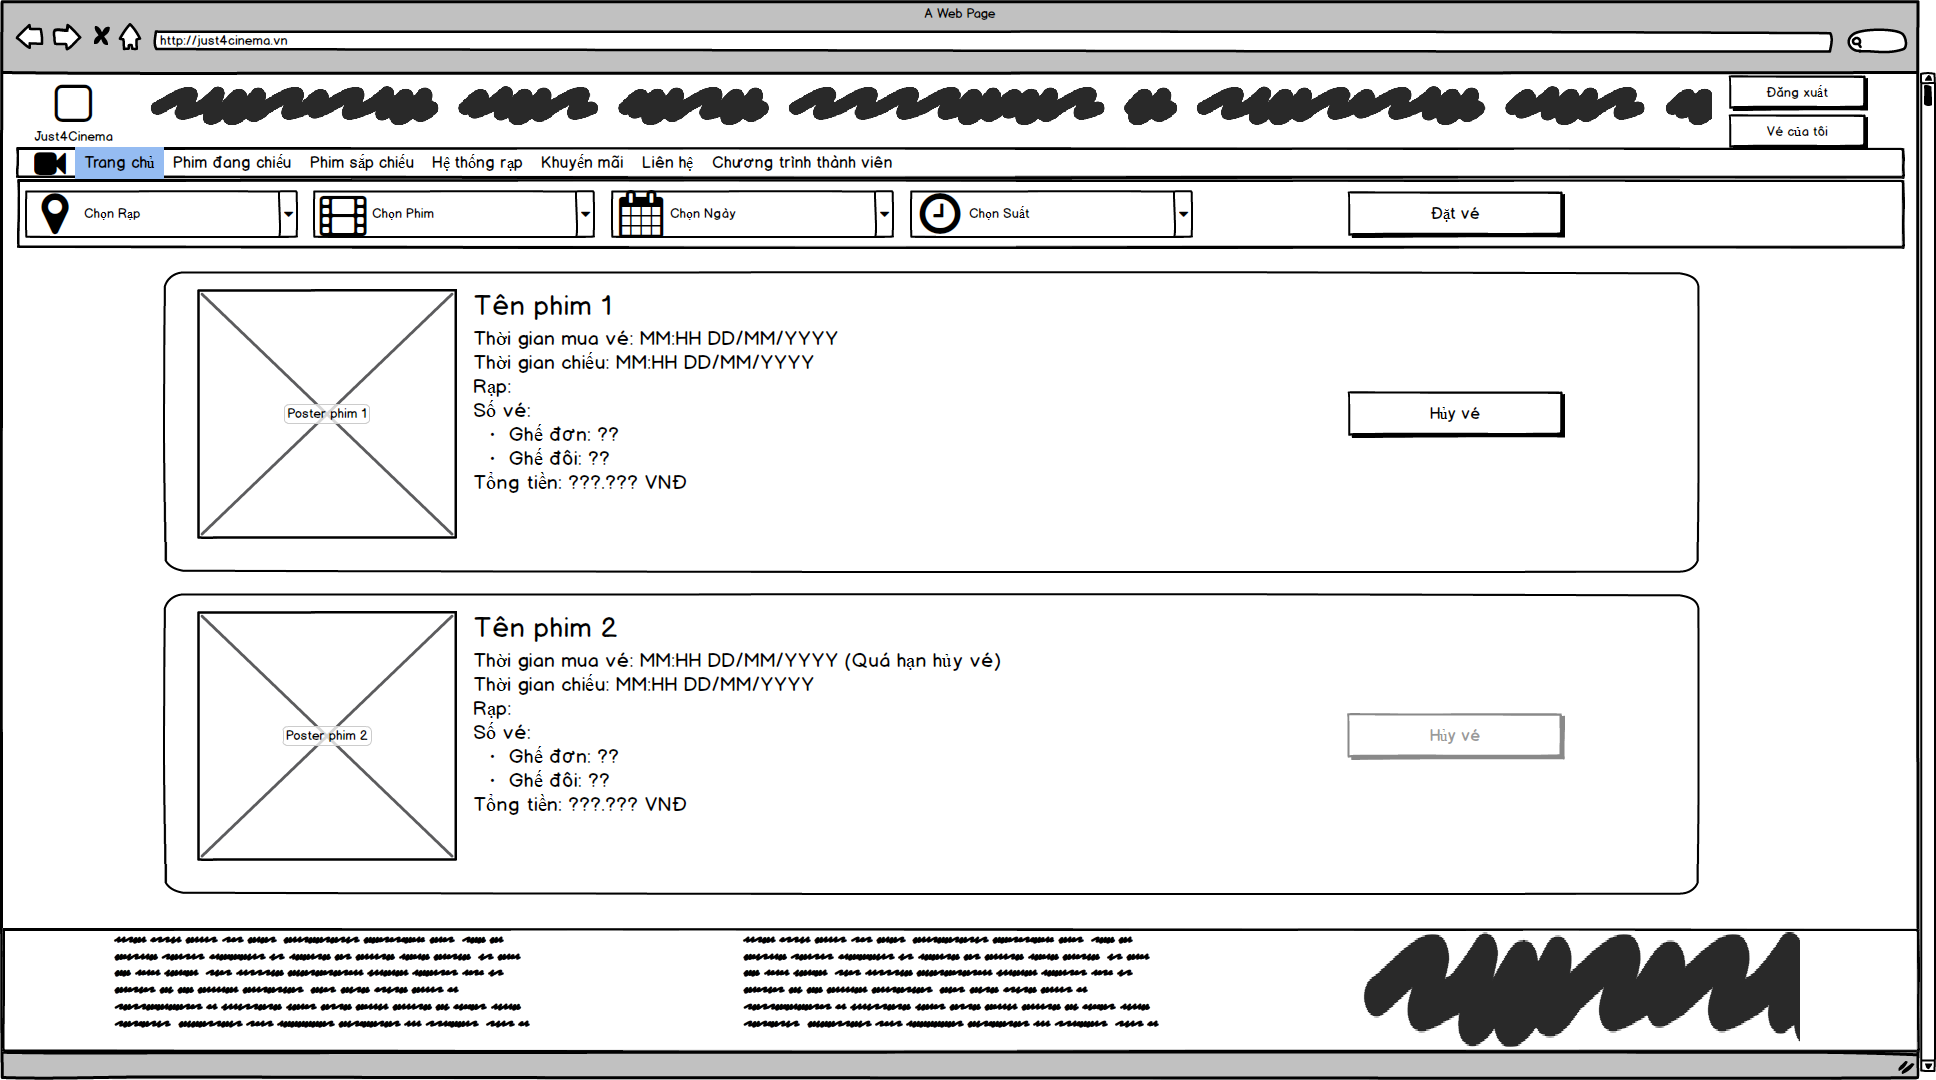
\includegraphics[scale = 0.25]{Wireframe/User/Vé của tôi.png}
                \caption{Giao diện hủy vé của khách hàng rạp phim}
            \end{center}
        \end{figure}

        %Use case Xem thông tin phim
        \item Use case Xem thông tin phim
        \begin{figure}[H]
            \begin{center}
                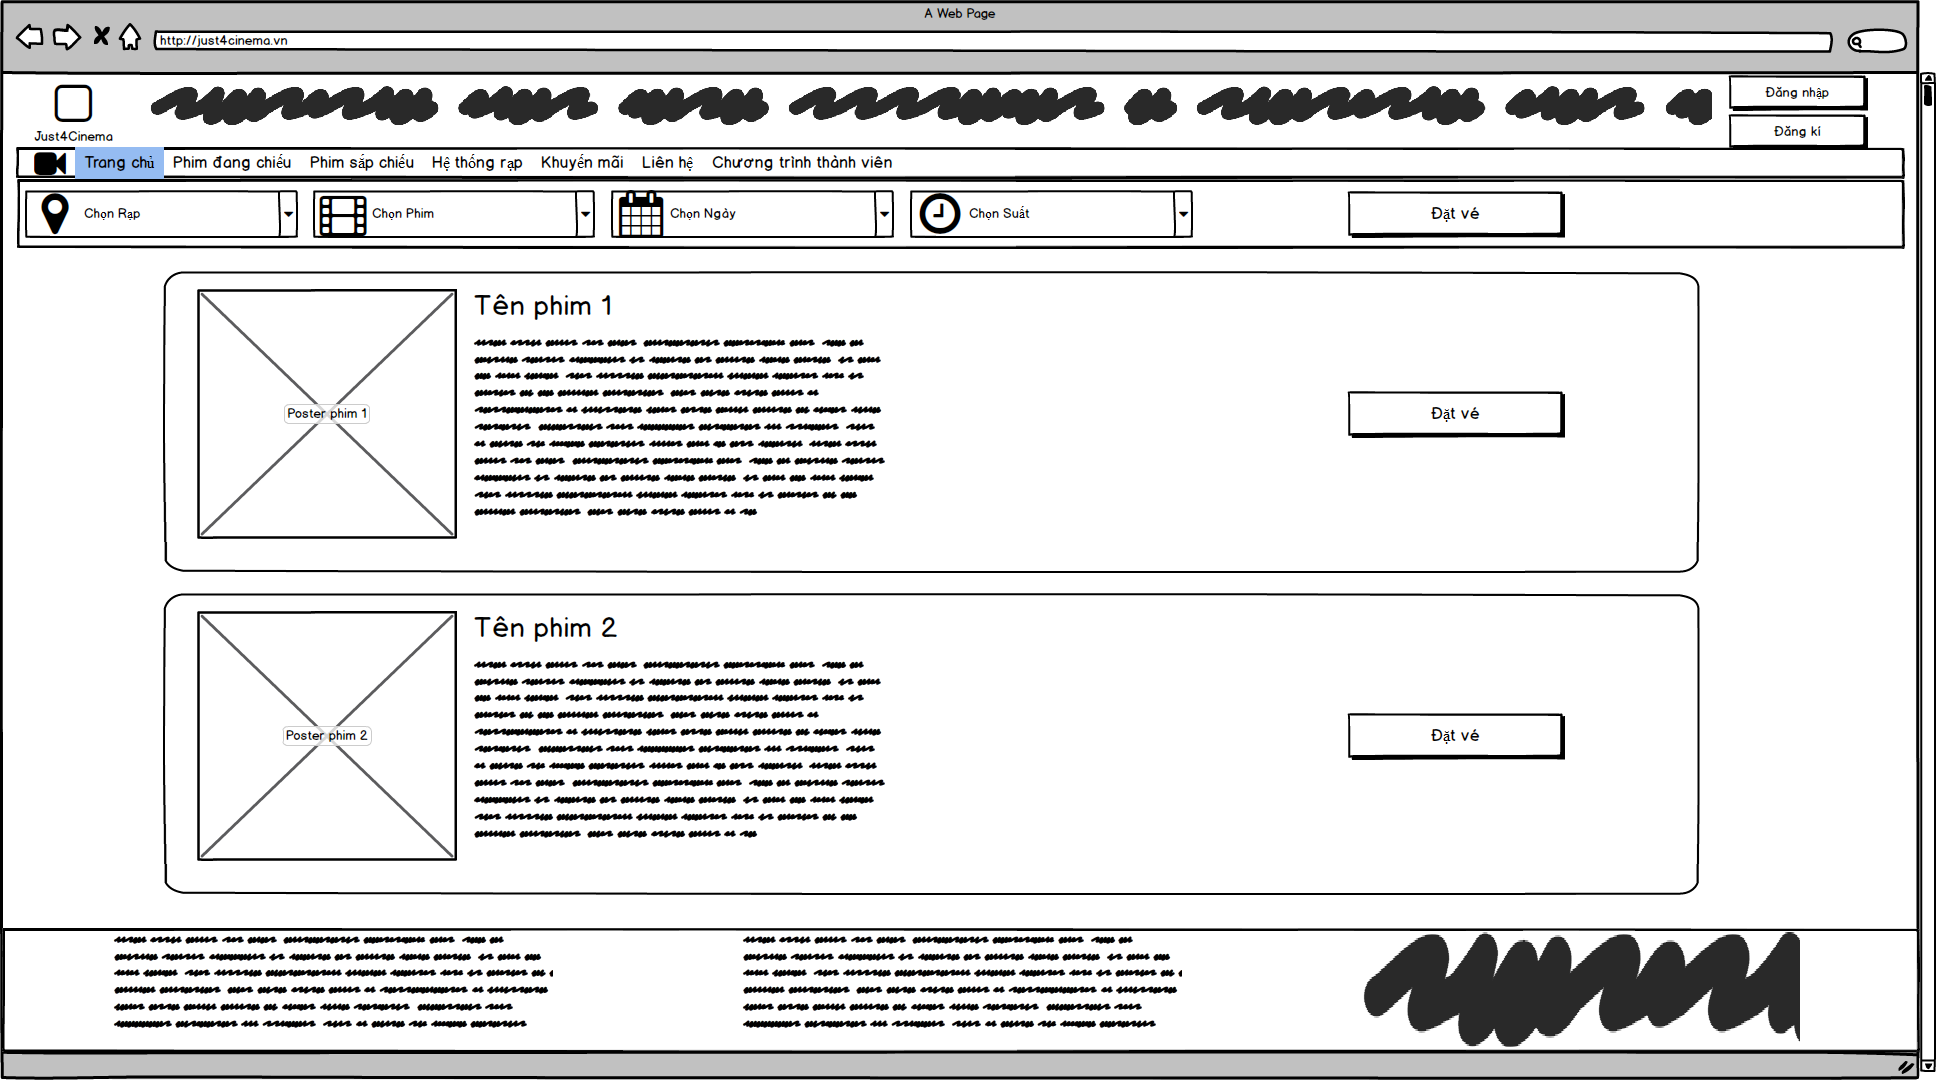
\includegraphics[scale = 0.25]{Wireframe/User/Phim đang chiếu_ Chọn phim.png}
                \caption{Giao diện xem thông tin phim}
            \end{center}
        \end{figure}

        %Use case Thanh toán online
        \item Use case Xem thông tin phim
        \begin{figure}[H]
            \begin{center}
                \includegraphics[scale = 0.25]{Wireframe/User/Thanh toán.png}
                \caption{Giao diện thanh toán online}
            \end{center}
        \end{figure}

        \begin{figure}[H]
            \begin{center}
                \includegraphics[scale = 0.25]{Wireframe/User/Thanh toán MOMO.png}
                \caption{Giao diện quét mã thanh toán}
            \end{center}
        \end{figure}

        %Use case Quản lý lịch chiếu
        \item Use case Xem thông tin phim
        \begin{figure}[H]
            \begin{center}
                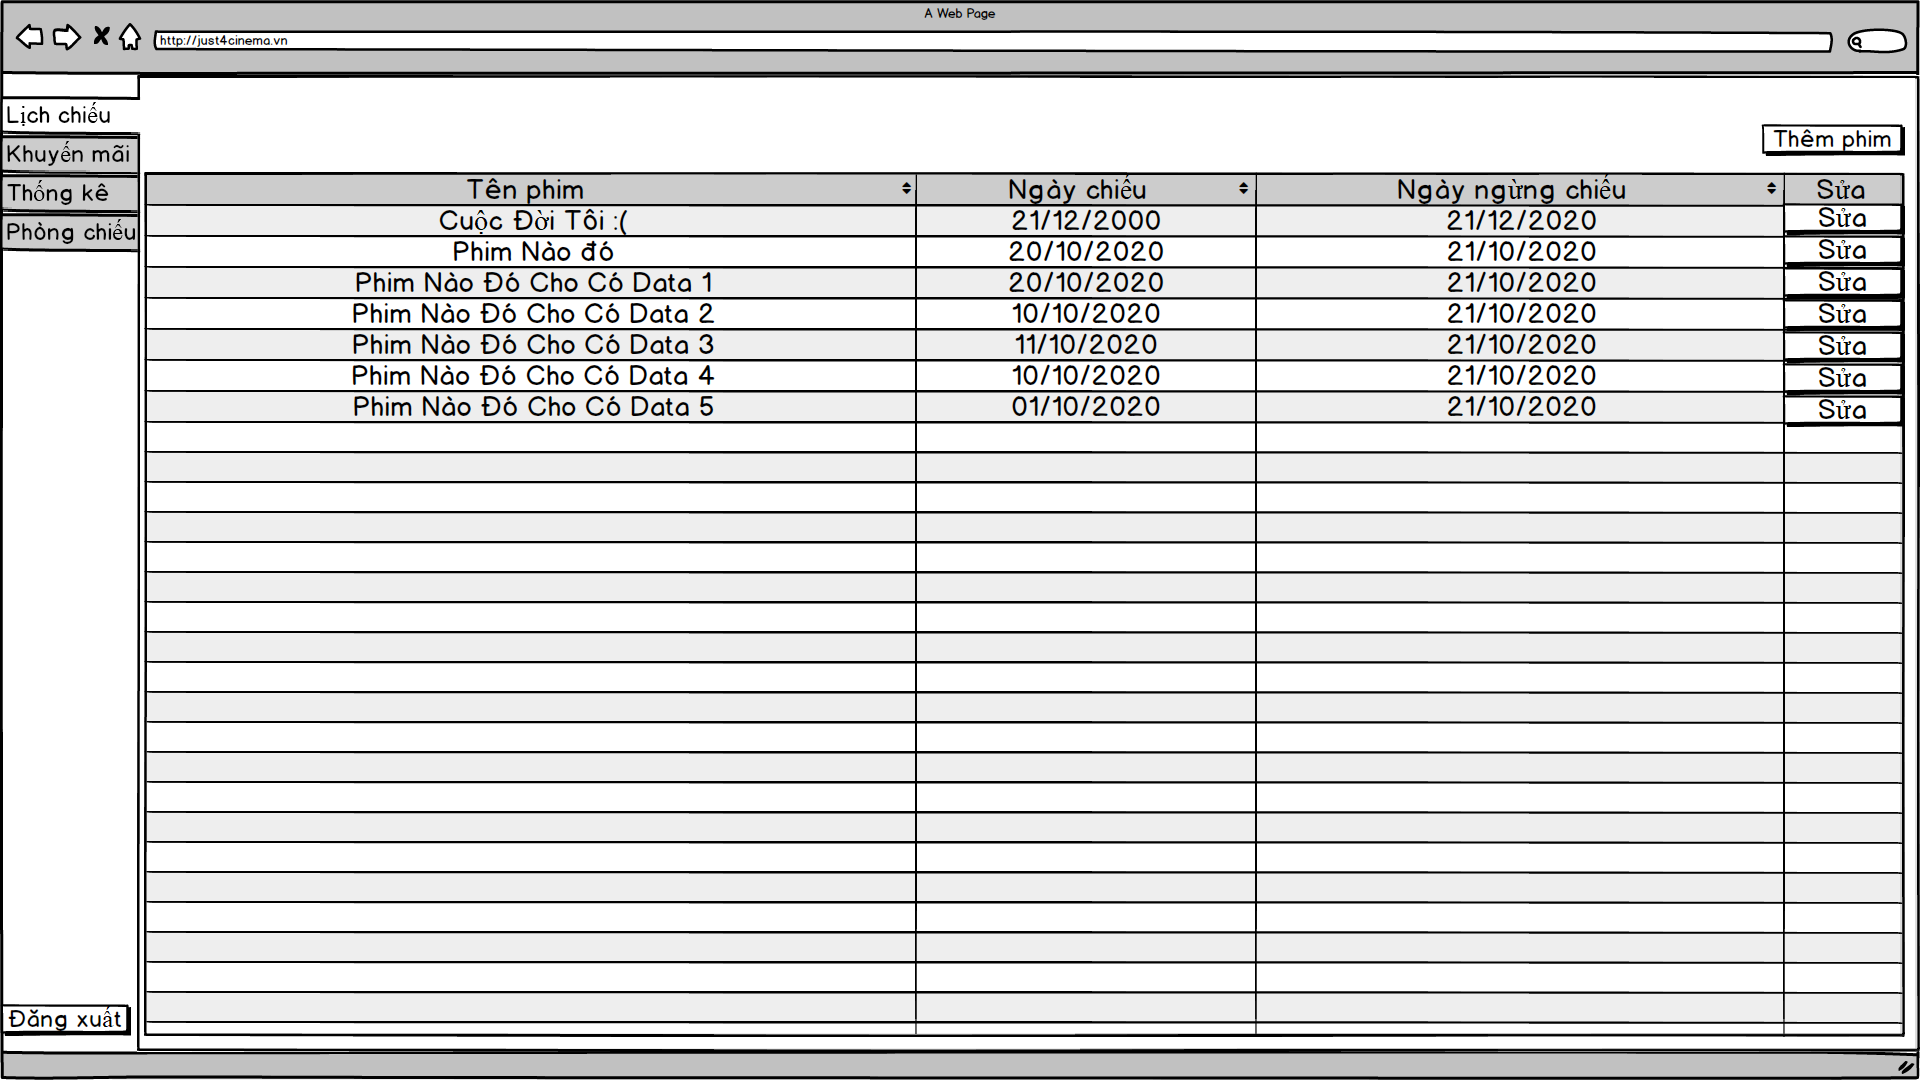
\includegraphics[scale = 0.25]{Wireframe/Manager/Quản lý_Dashboard_Lịch chiếu.png}
                \caption{Giao diện quản lý lịch chiếu}
            \end{center}
        \end{figure}

        \begin{figure}[H]
            \begin{center}
                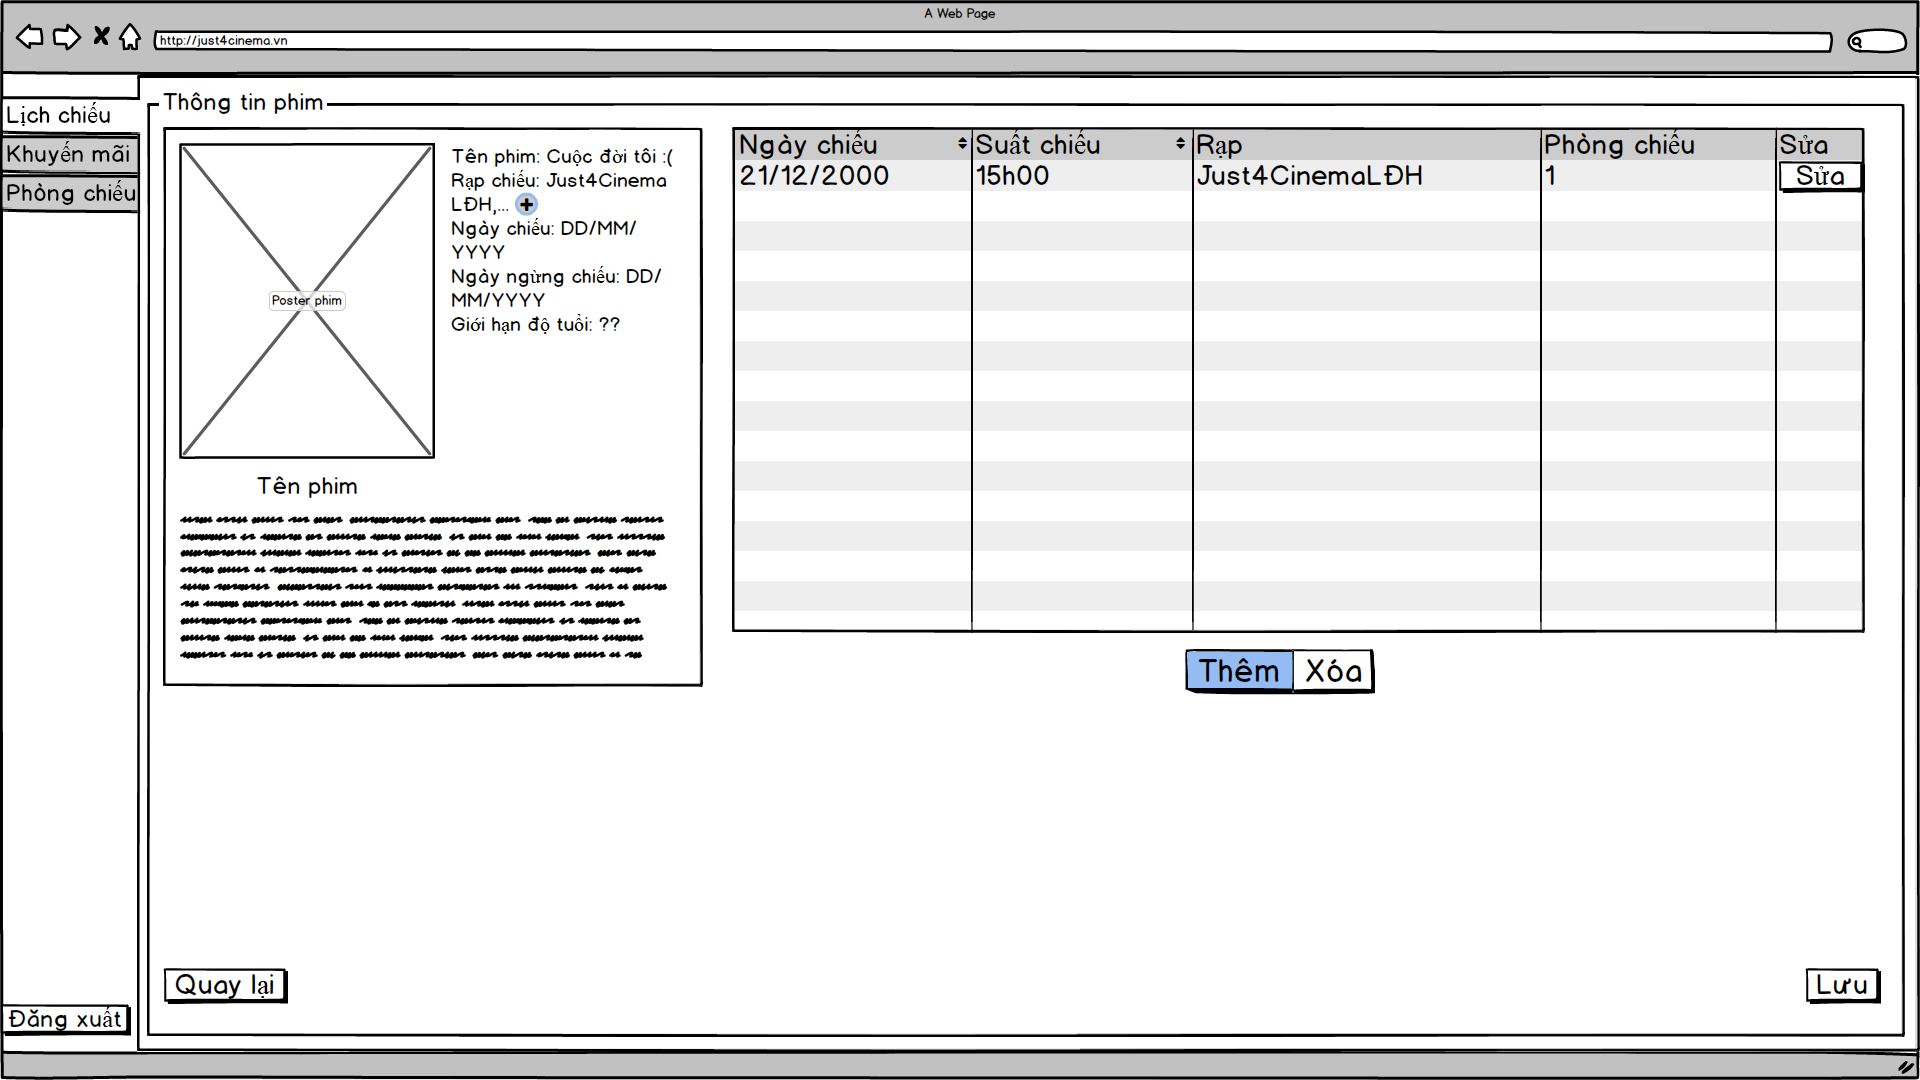
\includegraphics[scale = 0.25]{Wireframe/Manager/Quản lý_Dashboard_Sửa phim.png}
                \caption{Giao diện chỉnh sửa lịch chiếu}
            \end{center}
        \end{figure}

        %Use case Quản lý chương trình khuyến mãi
        \item Use case Xem thông tin phim
        \begin{figure}[H]
            \begin{center}
                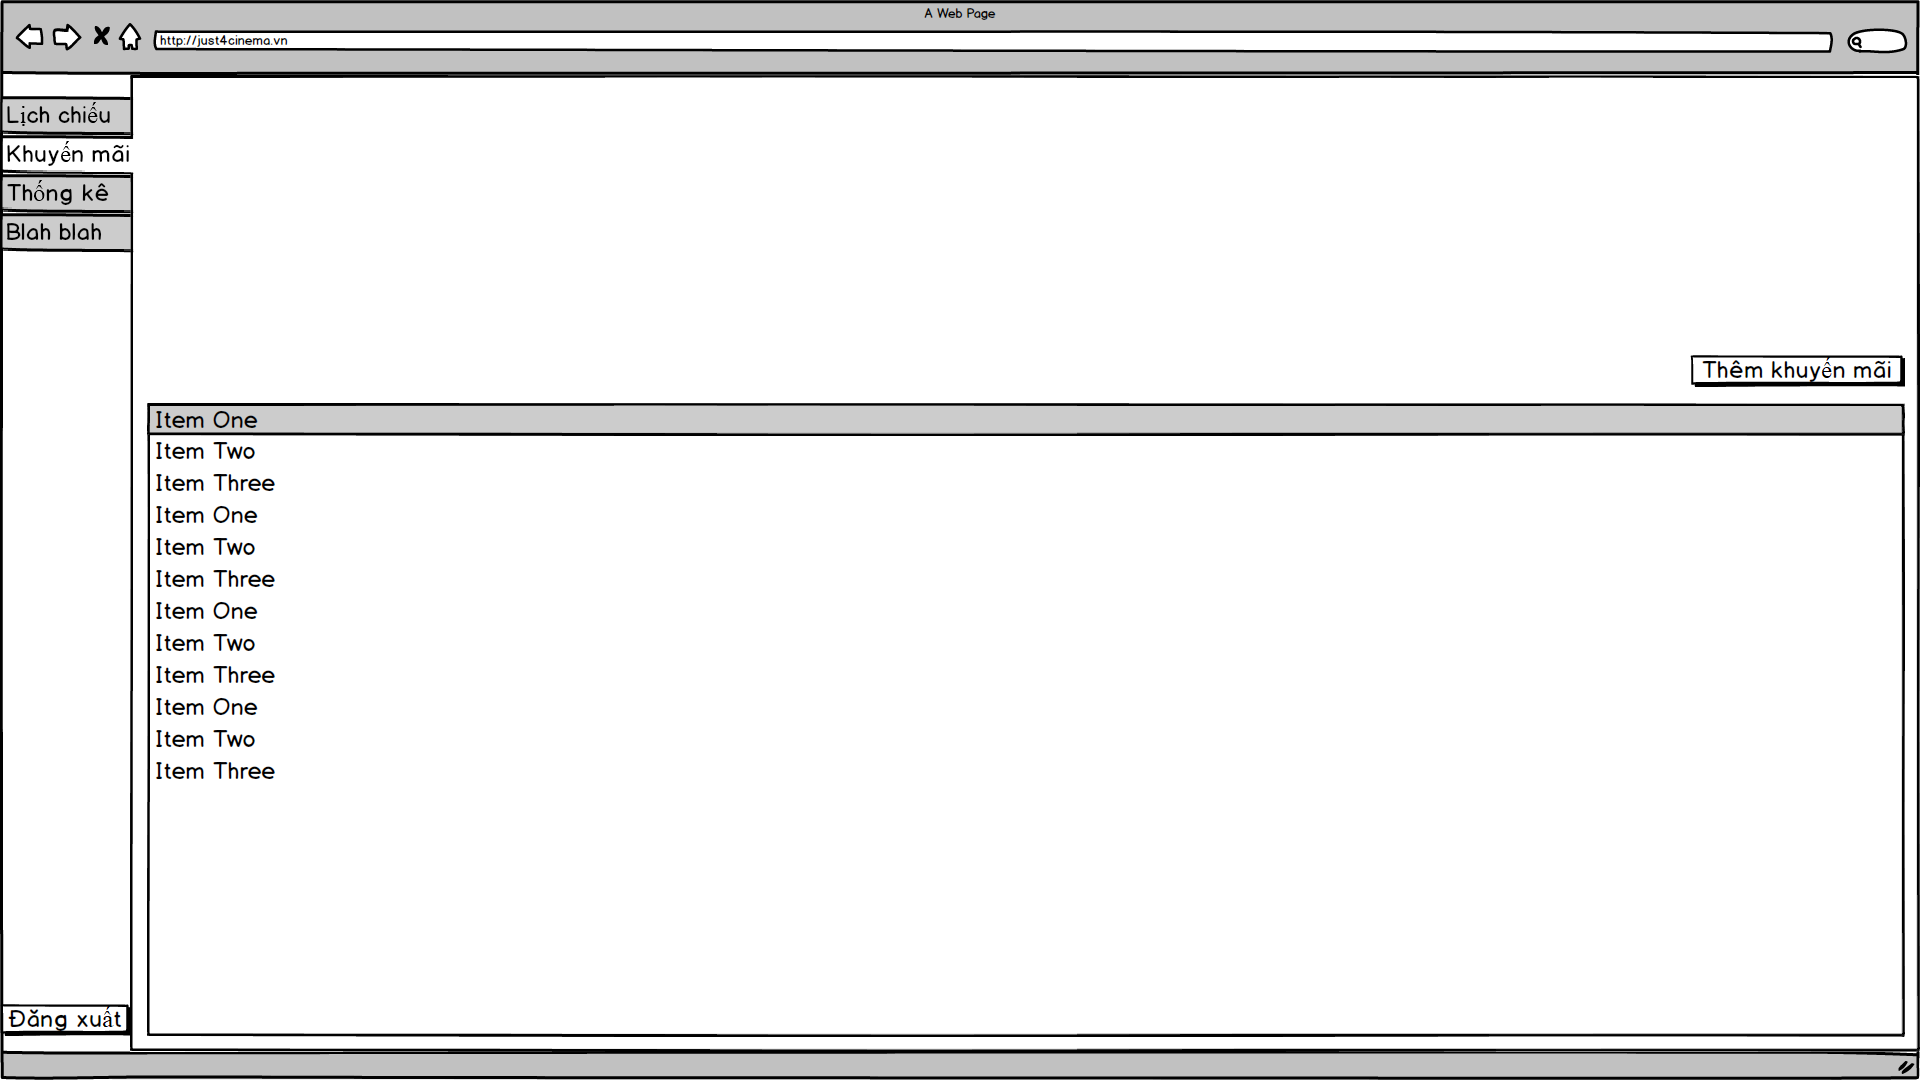
\includegraphics[scale = 0.25]{Wireframe/Manager/Quản lý_Dashboard_Khuyến mãi.png}
                \caption{Giao diện quản lý khuyến mãi}
            \end{center}
        \end{figure}

        \begin{figure}[H]
            \begin{center}
                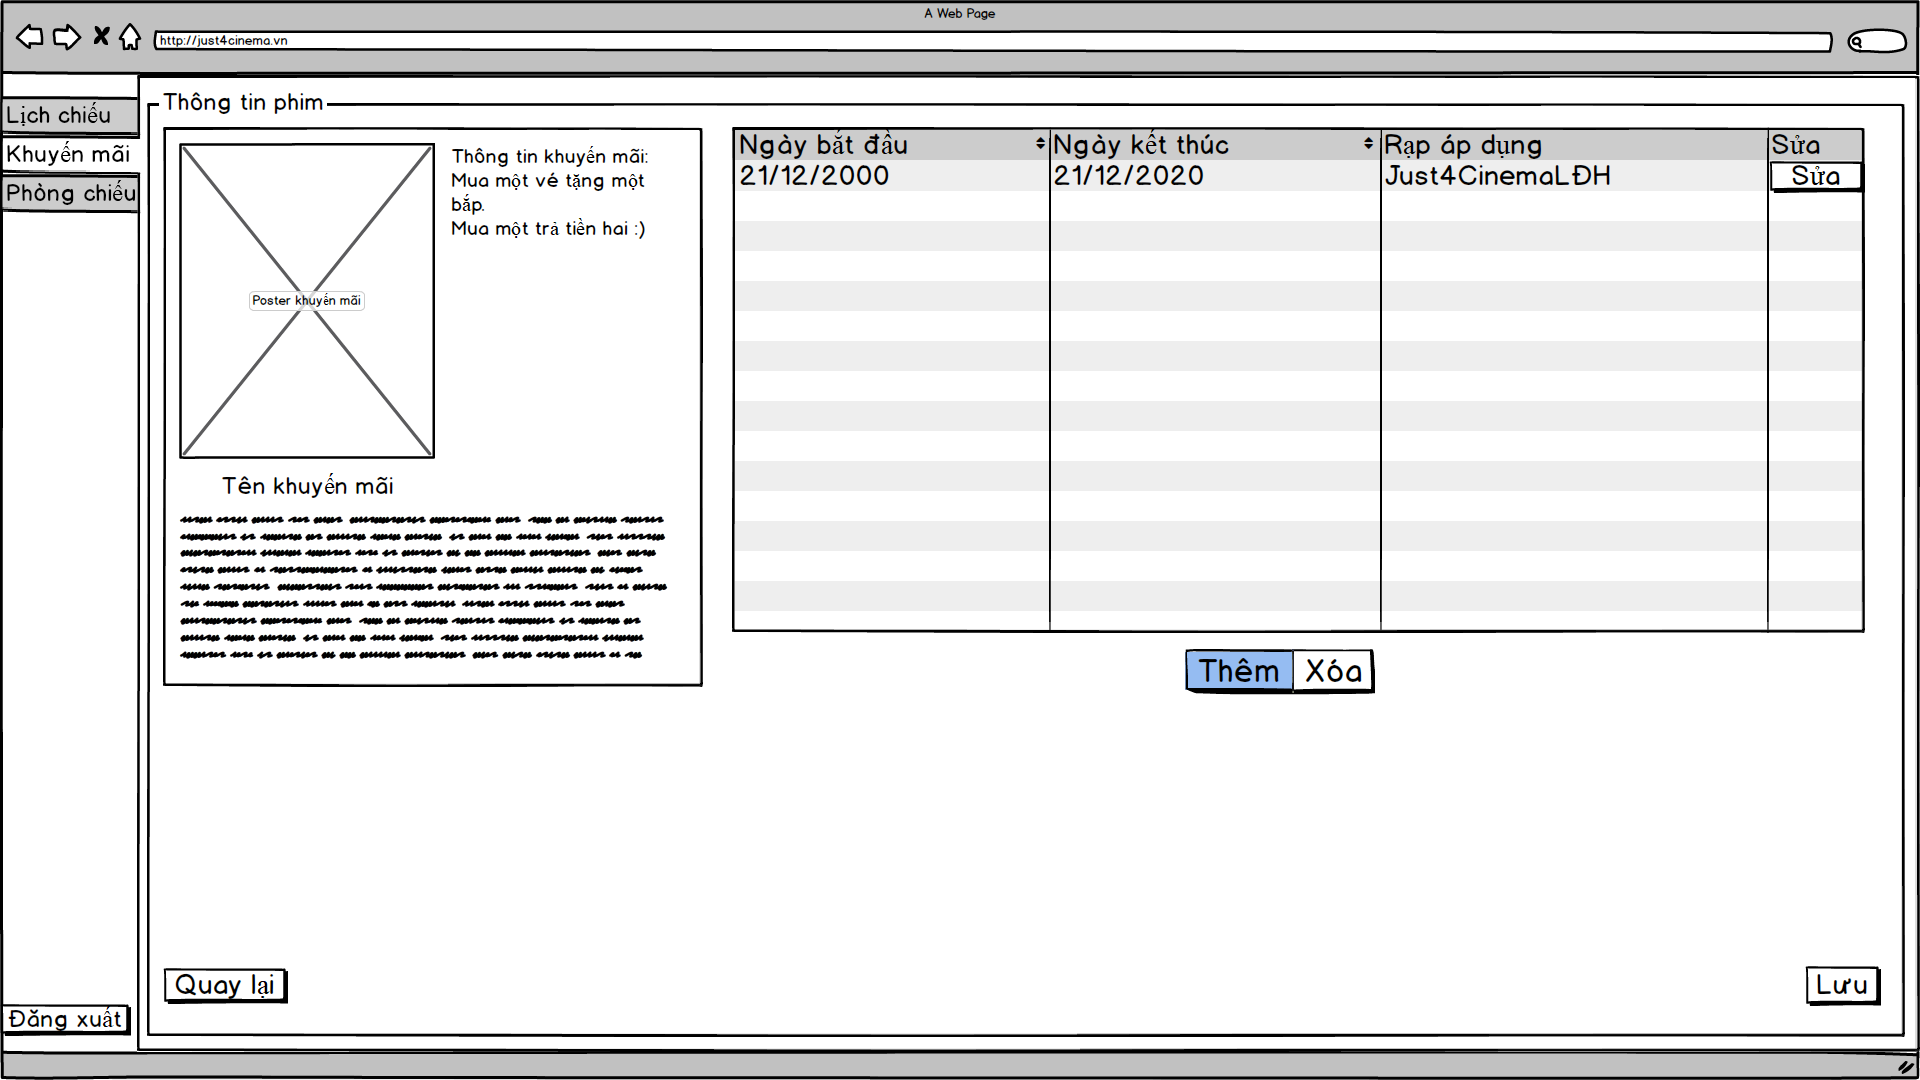
\includegraphics[scale = 0.25]{Wireframe/Manager/Quản lý_Dashboard_Sửa khuyến mãi.png}
                \caption{Giao diện chỉnh sửa khuyến mãi}
            \end{center}
        \end{figure}

        %Use case Quản lý các quản lý
        \item Use case Xem thông tin phim
        \begin{figure}[H]
            \begin{center}
                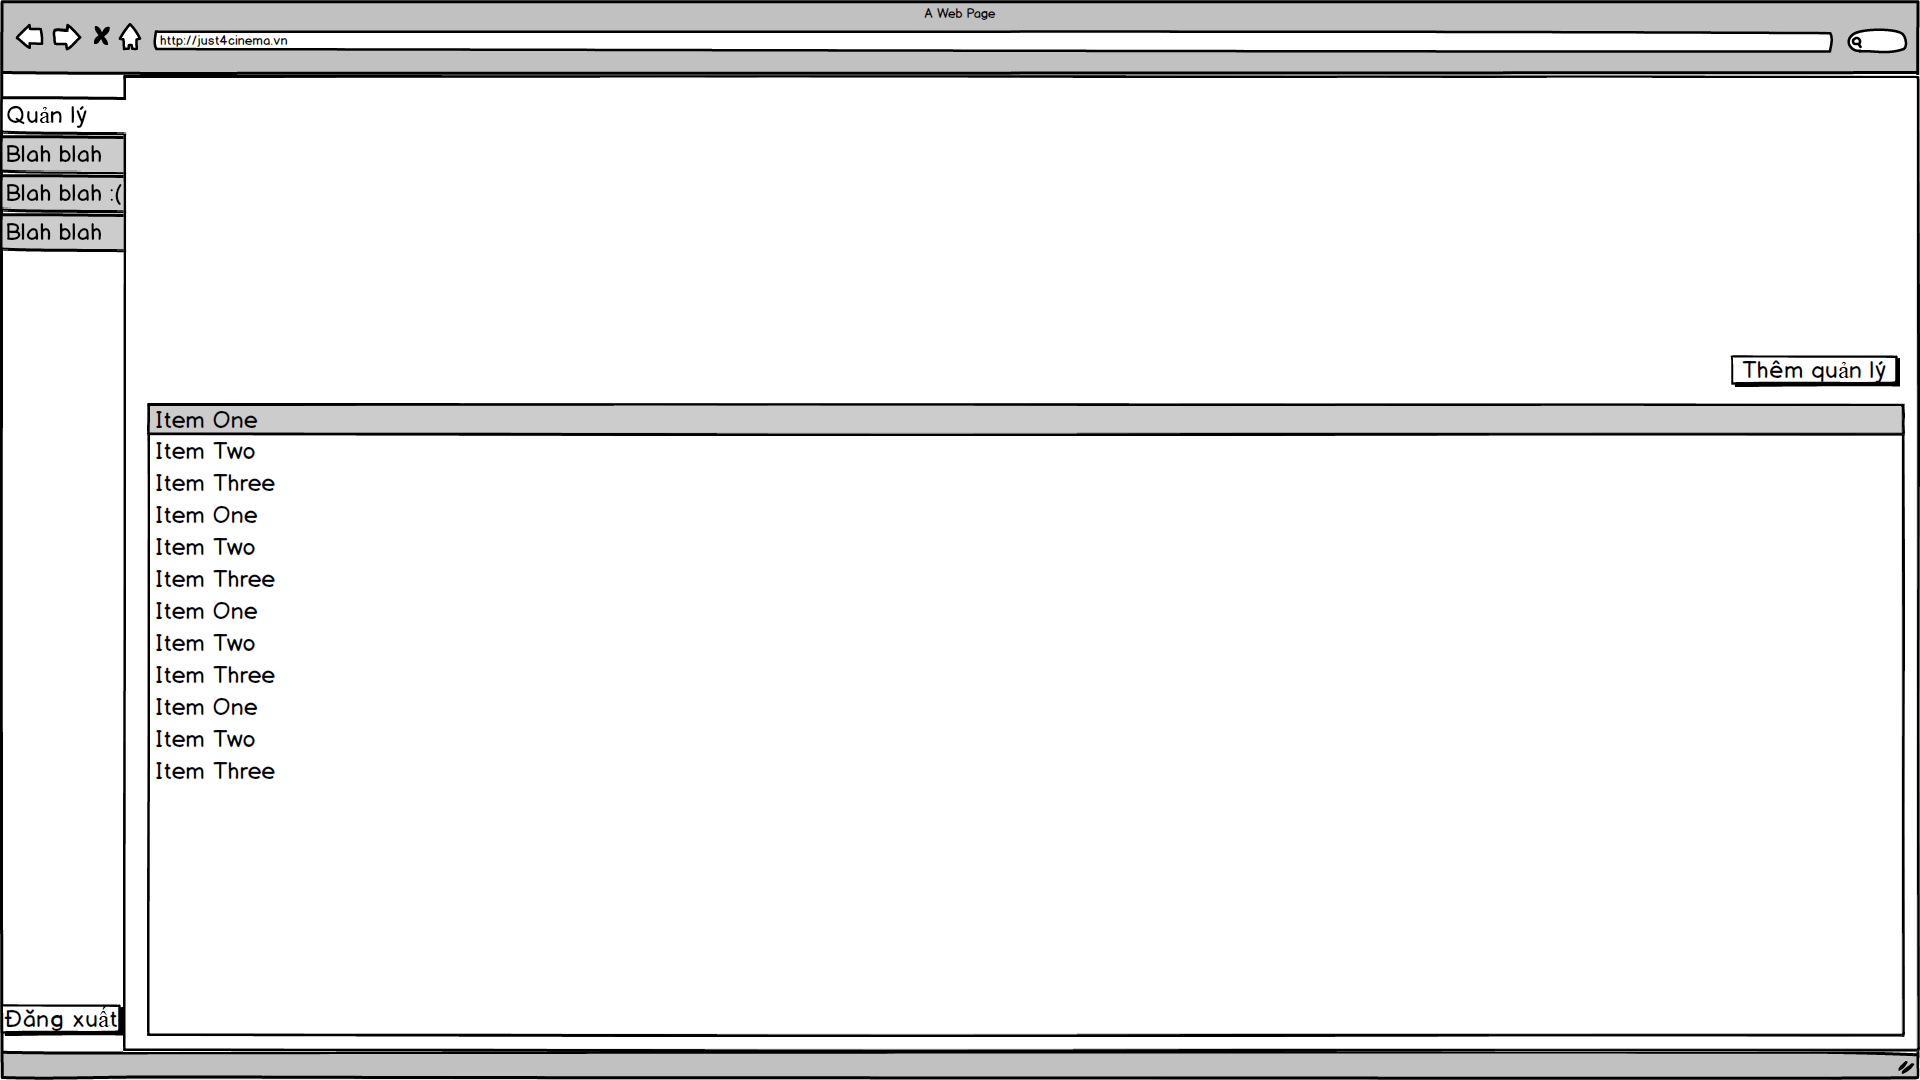
\includegraphics[scale = 0.25]{Wireframe/Admin/Admin_Quản lý.png}
                \caption{Giao diện quản lý các quản lý}
            \end{center}
        \end{figure}
        \begin{figure}[H]
            \begin{center}
                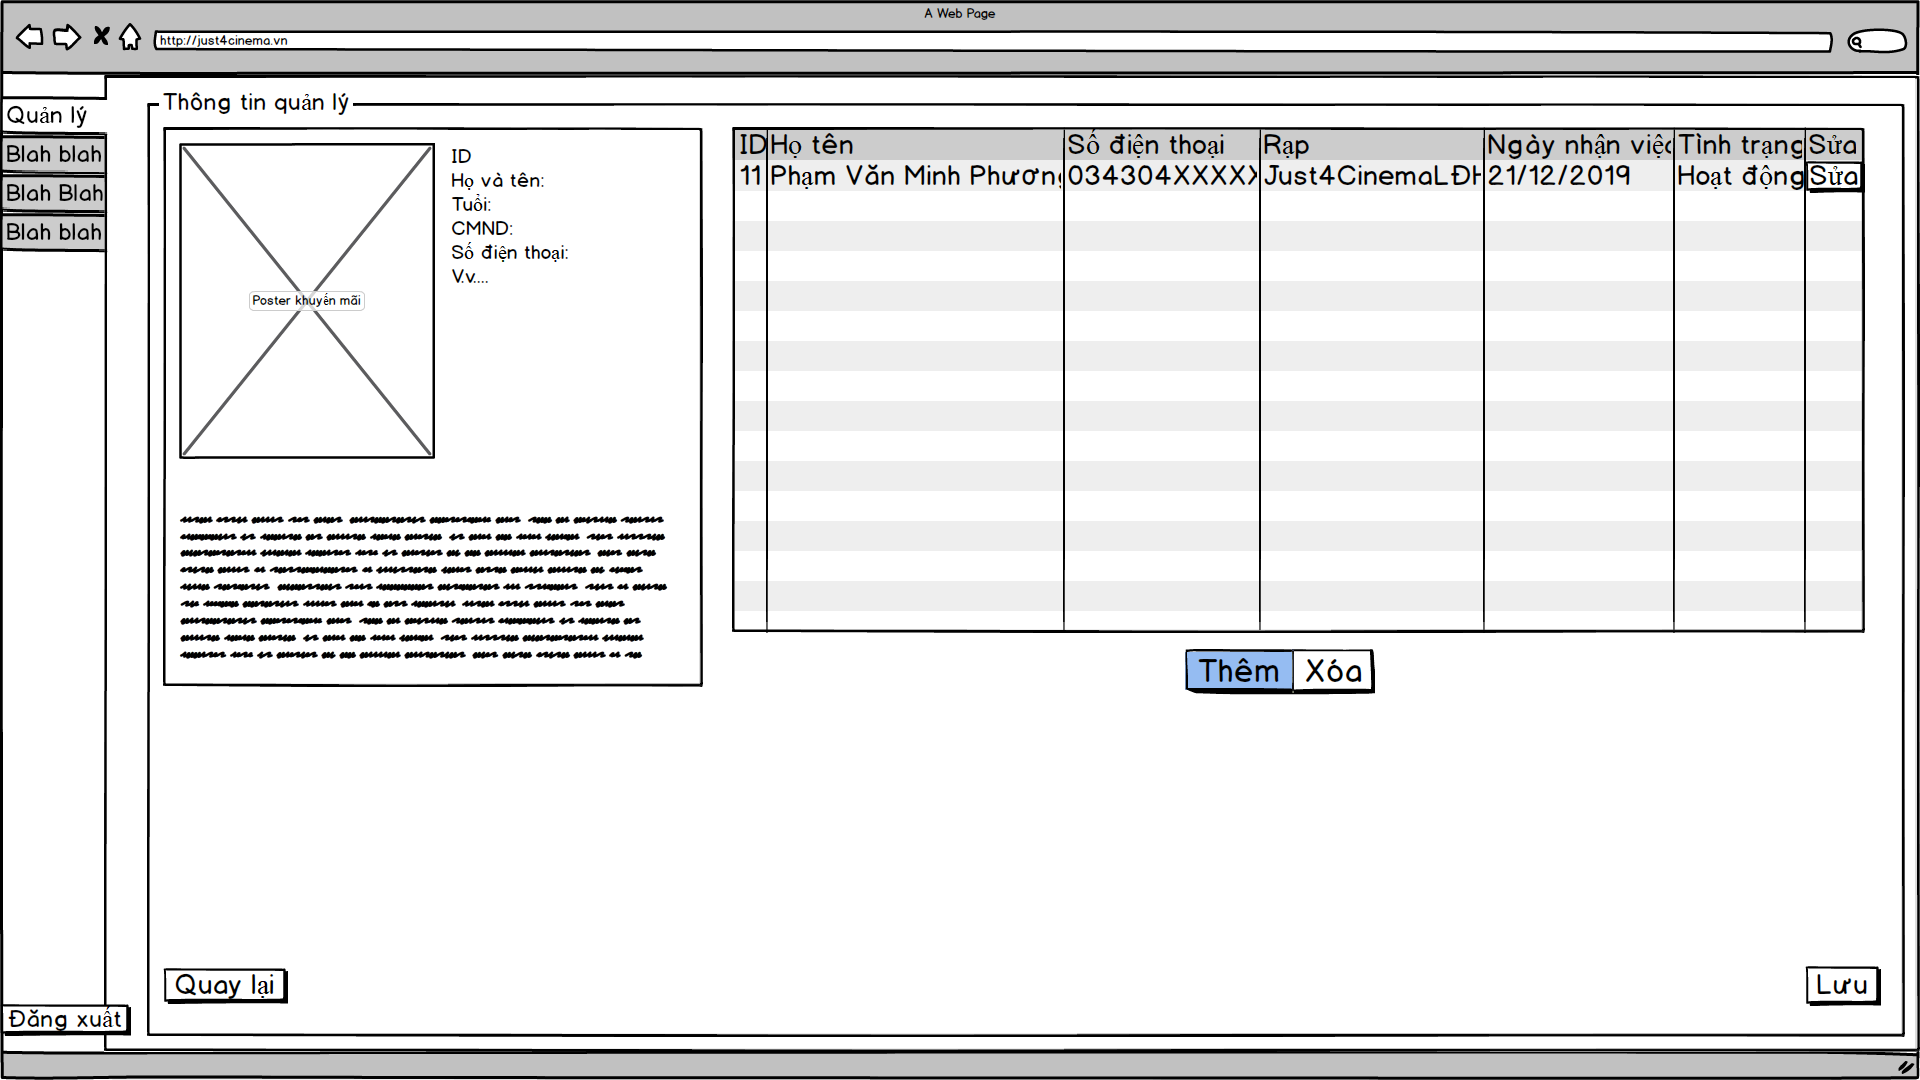
\includegraphics[scale = 0.25]{Wireframe/Admin/Admin_Hình quản lý.png}
                \caption{Giao diện chỉnh sửa một quản lý}
            \end{center}
        \end{figure}

        %Use case Thống kê doanh thu
        \item Use case Thống kê doanh thu
        \begin{figure}[H]
            \begin{center}
                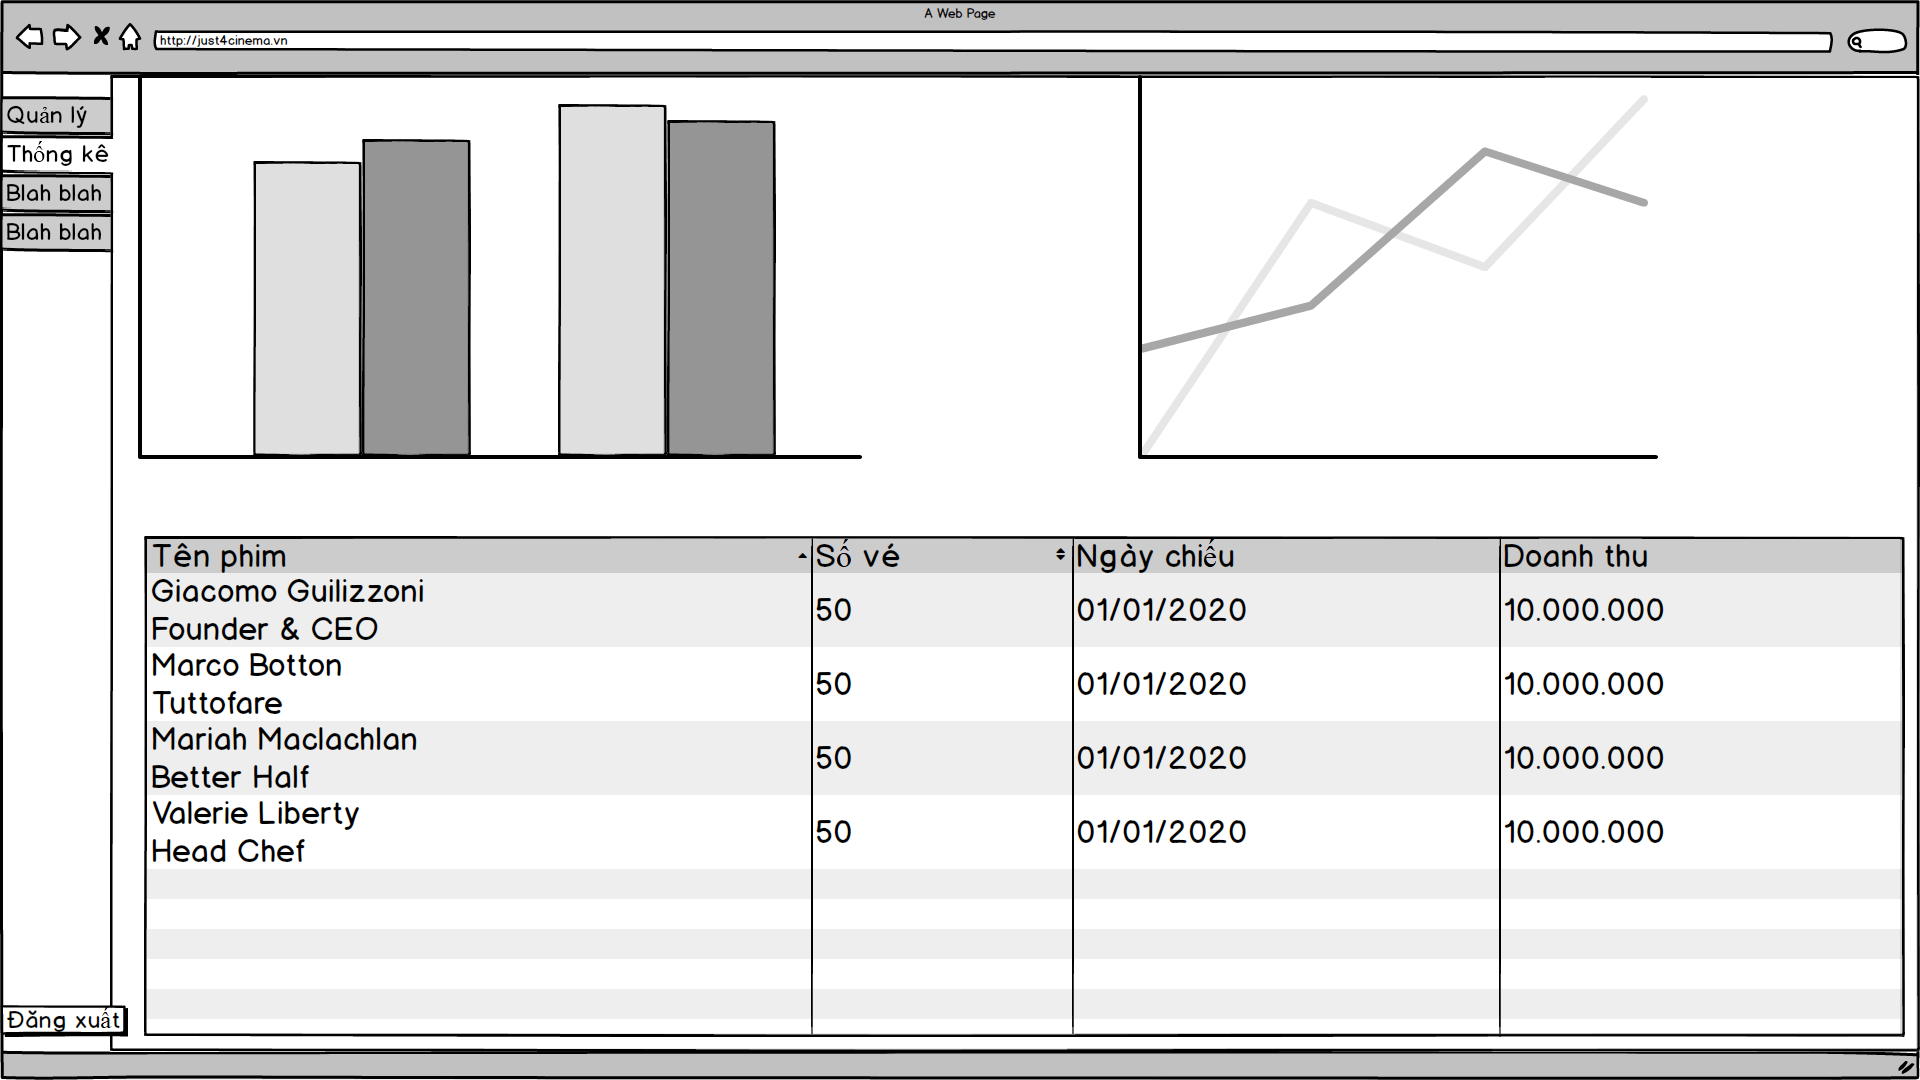
\includegraphics[scale = 0.25]{Wireframe/Admin/Admin_Thống kê.png}
                \caption{Giao diện thống kê doanh thu}
            \end{center}
        \end{figure}

    \end{enumerate}

    \subsection{Ước lượng nỗ lực người dùng}
    \begin{enumerate}
        \item Use case Đăng nhập
        \begin{itemize}
            % trong th k cần xuống dòng thì có thể xoá phần \begin{itemize} đi nhá 
            \item Khách hàng của rạp phim: Truy cập vào trang chủ, nhấn nút đăng nhập $\rightarrow$ Nhập thông tin, nhấn nút đăng nhập (2 bước, khoảng 4 lần click chuột, 2 lần nhập thông tin)
            \item Quản lý: Truy cập vào trang chủ, nhấn nút đăng nhập $\rightarrow$ Nhập thông tin, nhấn nút đăng nhập (2 bước, khoảng 4 lần click chuột, 2 lần nhập thông tin)
            \item Admin: Truy cập vào trang chủ, nhấn nút đăng nhập $\rightarrow$ Nhập thông tin, nhấn nút đăng nhập (2 bước, khoảng 4 lần click chuột, 2 lần nhập thông tin)
            \item Mất khoảng 10 giây để thực hiện các thao tác trên (Trong điều kiện lý tưởng)
        \end{itemize}

        %Use case Đăng kí
        \item Use case Đăng kí
        \begin{itemize}
            \item Khách hàng của rạp phim: Truy cập vào trang chủ, nhấn nút đăng kí $\rightarrow$ Nhập thông tin, nhấn nút đăng kí (2 bước, khoảng 12 lần click chuột, 9 lần nhập thông tin)
            \item Mất khoảng 2 phút để thực hiện các thao tác trên (Trong điều kiện lý tưởng)
        \end{itemize}

        %Use case Đăng xuất
        \item Use case Đăng kí
        \begin{itemize}
            \item Khách hàng của rạp phim: Nhấn nút đăng xuất (1 bước, 1 click)
            \item Quản lý: Nhấn nút đăng xuất (1 bước, 1 click)
            \item Admin: Nhấn nút đăng xuất (1 bước, 1 click)
            \item Mất 3 giây để thực hiện thao tác trên (Trong điều kiện lý tưởng)
        \end{itemize}

        %Use case Đặt vé
        \item Use case Đặt vé
        \begin{itemize}
            \item Khách hàng chọn thông tin về rạp, phim, ngày, suất chiếu tại thanh đặt vé nhanh, nhấn nút đặt vé $\rightarrow$ Điều chỉnh lại thông tin đặt vé nếu cần tại giao diện đặt vé, nhấn nút chọn ghế  $\rightarrow$ Chọn ghế, chuyển qua thanh toán (3 bước, khoảng 12 lần click chuột)
            \item Mất khoảng 2 phút để thực hiện các thao tác trên (Trong điều kiện lý tưởng)
        \end{itemize}

        %Use case Hủy vé
        \item Use case Hủy vé
        \begin{itemize}
            \item Khách hàng nhấn nút "Vé của tôi"  $\rightarrow$ Tìm và chọn vé muốn hủy, nhấn nút hủy vé $\rightarrow$ Nhấn xác nhận hủy vé (3 bước, khoảng 3 lần lick chuột)
            \item Mất khoảng 1 phút để thực hiện các thao tác trên (Trong điều kiện lý tưởng)
        \end{itemize}

        %Use case Xem thông tin phim
        \item Use case Xem thông tin phim
        \begin{itemize}
            \item Khách hàng nhấn nút "Phim đang chiếu"  $\rightarrow$ Tìm và chọn phim muốn xem thêm thông tin, nhấn xem thêm (2 bước, khoảng 2 lần click chuột)
            \item Mất khoảng 10 giây để thực hiện các thao tác trên (Trong điều kiện lý tưởng)
        \end{itemize}

        %Use case Thanh toán online
        \item Use case Thanh toán online
        \begin{itemize}
            \item Khách hàng sau khi chọn ghế nhấn nút "Thanh toán qua Momo" $\rightarrow$ Quét mã để hoàn thành thanh toán (2 bước, khoảng 2 lần click chuột)
            \item Mất khoảng 10 giây để thực hiện các thao tác trên (Trong điều kiện lý tưởng)
        \end{itemize}

        %Use case Quản lý lịch chiếu
        \item Use case Quản lý lịch chiếu 
        \begin{itemize}
            \item Quản lý sau khi đăng nhập vào dashboard, nhấn vào tab "Lịch chiếu" ở thanh công cụ bên trái $\rightarrow$ Danh sách phim đang chiếu hiện ra, nhấn "Thêm phim", nhập thông tin sơ bộ về phim, nhấn sửa $\rightarrow$ Danh sách các suất chiếu của một phim hiện ra, nhấn sửa để có thể thay đổi nội dung. (3 bước, khoảng 7 lần click chuột, 6 lần nhập thông tin cho mỗi phim cần thêm)
            \item Quản lý sau khi đăng nhập vào dashboard, nhấn vào tab "Lịch chiếu" ở thanh công cụ bên trái $\rightarrow$ Danh sách phim đang chiếu hiện ra, nhấn "Sửa" $\rightarrow$ Danh sách các suất chiếu của một phim hiện ra, nhấn sửa để có thể thay đổi nội dung. (3 bước, khoảng 7 lần click chuột cho mỗi phim cần sửa)
            \item Mất khoảng 2 phút để thực hiện các thao tác trên (Trong điều kiện lý tưởng)
        \end{itemize}

        %Use case Quản lý khuyến mãi
        \item Use case Quản lý khuyến mãi
        \begin{itemize}
            \item Quản lý sau khi đăng nhập vào dashboard, nhấn vào tab "Khuyến mãi" ở thanh công cụ bên trái $\rightarrow$ Danh sách khuyến mãi hiện ra, nhấn "Thêm khuyến mãi", nhập thông tin sơ bộ về khuyến mãi, nhấn sửa $\rightarrow$ Danh sách các rạp được áp dụng khuyến mãi hiện ra, nhấn sửa để có thể thay đổi nội dung. (3 bước, khoảng 7 lần click chuột, 3 lần nhập thông tin cho mỗi khuyến mãi cần thêm)
            \item Quản lý sau khi đăng nhập vào dashboard, nhấn vào tab "Khuyến mãi" ở thanh công cụ bên trái $\rightarrow$ Danh sách khuyến mãi hiện ra, nhấn "Sửa" , nhập thông tin sơ bộ về khuyến mãi, nhấn sửa $\rightarrow$ Danh sách các rạp được áp dụng khuyến mãi hiện ra, nhấn sửa để có thể thay đổi nội dung. (3 bước, khoảng 7 lần click chuột, 3 lần nhập thông tin cho mỗi khuyến mãi cần sửa)
            \item Mất khoảng 2 phút để thực hiện các thao tác trên (Trong điều kiện lý tưởng)
        \end{itemize}

        %Use case Quản lý các quản lý
        \item Use case Quản lý các quản lý
        \begin{itemize}
            \item Admin sau khi đăng nhập vào dashboard, nhấn vào tab "Quản lý" ở thanh công cụ bên trái $\rightarrow$ Danh sách quản lý hiện ra, nhấn "Thêm quản lý" $\rightarrow$ Danh sách các quản lý hiện ra, nhấn sửa để có thể thay đổi nội dung. (2 bước, khoảng 7 lần click chuột, 4 lần nhập thông tin cho mỗi quản lý cần thêm)
            \item Admin sau khi đăng nhập vào dashboard, nhấn vào tab "Quản lý" ở thanh công cụ bên trái $\rightarrow$ Danh sách quản lý hiện ra, nhấn "Sửa" $\rightarrow$ Danh sách các quản lý hiện ra, nhấn sửa để có thể thay đổi nội dung. (2 bước, khoảng 7 lần click chuột, 4 lần nhập thông tin cho mỗi quản lý cần thêm)
            \item Mất khoảng 2 phút để thực hiện các thao tác trên (Trong điều kiện lý tưởng)
        \end{itemize}

        %Use case Thống kê doanh thu
        \item Use case Thống kê doanh thu
        \begin{itemize}
            \item Admin sau khi đăng nhập vào dashboard, nhấn vào tab "Thống kê" ở thanh công cụ bên trái $\rightarrow$ Giao diện thống kê hiện ra, có thể chọn thống kê theo các tiêu chí khác nhau (2 bước, khoảng 4 lần click chuột)
            \item Mất khoảng 30 giây để thực hiện các thao tác trên (Trong điều kiện lý tưởng)
        \end{itemize}
    \end{enumerate}
    \clearpage

    \section{Kế hoạch làm việc}
    \label{sec:plan}

    \subsection{Các mốc milestone}
    \begin{table}[H]
        \begin{tabular}{|c|c|l|}
        \hline
        STT & MilestoneID & \multicolumn{1}{c|}{Nội dung}             \\ \hline
        1   & M1          & Nộp báo cáo Phân tích thiết kế hệ thống   \\ \hline
        2   & M2          & Nộp báo cáo Giao diện và kiểm thử         \\ \hline
        3   & M3          &\begin{tabular}[c]{@{}l@{}}Demo version 1:\\ Yêu cầu 2.3 (Quản lý thông tin phim)\\ Yêu cầu 1.4 (Đặt vé)\\ Yêu cầu 1.5 (Huỷ vé)\end{tabular} \\ \hline
        4   & M4          &\begin{tabular}[c]{@{}l@{}}Demo version 2\\ Yêu cầu 1.7 (Thanh toán online) \\ Yêu cầu 1.6 (Xem thông tin phim)\\ Yêu cầu 1.1 (Đăng ký tài khoản)\\ Yêu cầu 1.2, 2.1, 3.1 (Đăng nhập của khách của rạp, quản lý, admin)\\ Yêu cầu 1.3, 2.2, 3.2 (Đăng xuất của khách của rạp, quản lý, admin)\end{tabular} \\ \hline
        5   & M5          &\begin{tabular}[c]{@{}l@{}}Demo version 3:\\ Yêu cầu 3.3 (Quản lý các quản lý của rạp phim)\\ Yêu cầu 2.4 (Quản lý chương trình khuyến mãi)\\ Yêu cầu 3.4(Thực hiện các thống kê doanh thu)\end{tabular} \\ \hline
        6   & M6          & Nộp báo cáo Cuối kỳ                       \\ \hline
        7   & M7          & Vấn đáp Đồ án cuối kỳ (Thực hành cuối kỳ) \\ \hline
        \end{tabular}
        \caption{Bảng các mốc milestone của dự án}
    \end{table}

    \subsection{Tác vụ cần thực hiện}
    \begin{table}[H]
        \begin{center}
            \begin{tabular}{|c|c|l|}
            \hline
            STT & Task ID & \multicolumn{1}{c|}{Nội dung}                               \\ \hline \rowcolor[HTML]{E6B8AF} 
            1   & T1      & Thực hiện báo cáo Phân tích thiết kế Hệ thống               \\ \hline \rowcolor[HTML]{EAD1DC} 
            2   & T2      & Thực hiện báo cáo Giao diện và kiểm thử                     \\ \hline \rowcolor[HTML]{D9EAD3} 
            3   & T3      & Cài đặt yêu cầu 2.3 (Quản lý thông tin phim)                \\ \hline \rowcolor[HTML]{D9EAD3} 
            4   & T4      & Cài đặt yêu cầu 1.4 (Đặt vé)                                \\ \hline \rowcolor[HTML]{D9EAD3} 
            5   & T5      & Cài đặt yêu cầu 1.5 (Hủy vé)                                \\ \hline \rowcolor[HTML]{FFFFFF} 
            6   & T6      & Cài đặt yêu cầu 1.7 (Thanh toán online)                     \\ \hline \rowcolor[HTML]{FFFFFF} 
            7   & T7      & Cài đặt yêu cầu 1.6 (Xem thông tin phim)                    \\ \hline \rowcolor[HTML]{FFFFFF} 
            8   & T8      & Cài đặt yêu cầu 1.1 (Đăng ký tài khoản)                     \\ \hline \rowcolor[HTML]{FFFFFF} 
            9   & T9      & Cài đặt yêu cầu 1.2 (Đăng nhập cho khách hàng của rạp phim) \\ \hline \rowcolor[HTML]{FFFFFF} 
            10  & T10     & Cài đặt yêu cầu 2.1 (Đăng nhập cho quản lý của rạp phim)    \\ \hline \rowcolor[HTML]{FFFFFF} 
            11  & T11     & Cài đặt yêu cầu 3.1 (Đăng nhập cho admin)                   \\ \hline \rowcolor[HTML]{FFFFFF} 
            12  & T12     & Cài đặt yêu cầu 1.3 (Đăng xuất cho khách hàng của rạp phim) \\ \hline \rowcolor[HTML]{FFFFFF} 
            13  & T13     & Cài đặt yêu cầu 2.2 (Đăng xuất cho quản lý)                 \\ \hline \rowcolor[HTML]{FFFFFF} 
            14  & T14     & Cài đặt yêu cầu 3.2 (Đăng xuất cho admin)                   \\ \hline \rowcolor[HTML]{C9DAF8} 
            15  & T15     & Cài đặt yêu cầu 3.3 (Quản lý các quản lý cho admin)         \\ \hline \rowcolor[HTML]{C9DAF8} 
            16  & T16     & Cài đặt yêu cầu 2.4 (Quản lý chương trình khuyến mãi)       \\ \hline \rowcolor[HTML]{C9DAF8} 
            17  & T17     & Cài đặt yêu cầu 3.4 (Thực hiện thống kê cho admin)          \\ \hline \rowcolor[HTML]{FCE5CD} 
            18  & T18     & Thực hiện báo cáo cuối kỳ                                   \\ \hline \rowcolor[HTML]{D0E0E3} 
            19  & T19     & Thực hiện vấn đáp cuối kỳ                                   \\ \hline
            \end{tabular}
            \caption{Bảng nội dung các tác vụ cần thực hiện trong dự án}
        \end{center}
    \end{table}

    \subsection{Thời gian thực hiện tác vụ và phụ thuộc tác vụ}
    \begin{table}[H]
        \begin{center}
            \begin{tabular}{|c|c|c|l|}
            \hline
            Task ID & Effort (person-days) & Duration (days) & \multicolumn{1}{c|}{Dependencies}                               \\ \hline \rowcolor[HTML]{E6B8AF} 
            T1      & 70                   & 14              & \\ \hline \rowcolor[HTML]{EAD1DC} 
            T2      & 70                   & 14              &T1(M1) \\ \hline \rowcolor[HTML]{D9EAD3} 
            T3      & 10                   & 10              &T2(M2) \\ \hline \rowcolor[HTML]{D9EAD3} 
            T4      & 28                   & 14              &T2(M2) \\ \hline \rowcolor[HTML]{D9EAD3} 
            T5      & 20                   & 10              &T2(M2) \\ \hline \rowcolor[HTML]{FFFFFF} 
            T6      & 14                   & 14              &T4(M3) \\ \hline \rowcolor[HTML]{FFFFFF} 
            T7      & 13                   & 13              &T4(M3) \\ \hline \rowcolor[HTML]{FFFFFF} 
            T8      & 13                   & 13              &T4(M3) \\ \hline \rowcolor[HTML]{FFFFFF} 
            T9      & 4                    & 4               &T4(M3) \\ \hline \rowcolor[HTML]{FFFFFF} 
            T10     & 4                    & 4               &T4(M3) \\ \hline \rowcolor[HTML]{FFFFFF} 
            T11     & 4                    & 4               &T4(M3) \\ \hline \rowcolor[HTML]{FFFFFF} 
            T12     & 4                    & 4               &T4(M3) \\ \hline \rowcolor[HTML]{FFFFFF} 
            T13     & 4                    & 4               &T4(M3) \\ \hline \rowcolor[HTML]{FFFFFF} 
            T14     & 4                    & 4               &T4(M3) \\ \hline \rowcolor[HTML]{C9DAF8} 
            T15     & 7                    & 6               &T6(M4) \\ \hline \rowcolor[HTML]{C9DAF8} 
            T16     & 7                    & 6               &T6(M4) \\ \hline \rowcolor[HTML]{C9DAF8} 
            T17     & 21                   & 7               &T6(M4) \\ \hline \rowcolor[HTML]{FCE5CD} 
            T18     & 70                   & 14              &T17(M5) \\ \hline \rowcolor[HTML]{D0E0E3} 
            T19     & 5                    & 1               &T18(M6) \\ \hline
            \end{tabular}
            \caption{Bảng nội dung các tác vụ cần thực hiện trong dự án}
        \end{center}
    \end{table}
    % \begin{table}[H]
    %     \begin{tabular}{|c|c|c|l|} \hline
    %     ID yêu cầu & Effort(person của days) & Duration(days)     & \multicolumn{1}{c|}{Dependencies} \\ \hline \rowcolor[HTML]{E6B8AF} 
    %     T1  & 70 & 14 &         \\ \hline \rowcolor[HTML]{EAD1DC} 
        % T2  & 70 & 14 & T1(M1)  \\ \hline \rowcolor[HTML]{D9EAD3} 
        % T3  & 10 & 10 & T2(M2)  \\ \hline \rowcolor[HTML]{D9EAD3} 
        % T4  & 28 & 14 & T2(M2)  \\ \hline \rowcolor[HTML]{D9EAD3} 
        % T5  & 20 & 10 & T2(M2)  \\ \hline \rowcolor[HTML]{FFFFFF} 
        % T6  & 14 & 14 & T4(M3)  \\ \hline \rowcolor[HTML]{FFFFFF} 
        % T7  & 13 & 13 & T4(M3)  \\ \hline \rowcolor[HTML]{FFFFFF} 
        % T8  & 13 & 13 & T4(M3)  \\ \hline \rowcolor[HTML]{FFFFFF} 
        % T9  & 4  & 4  & T4(M3)  \\ \hline \rowcolor[HTML]{FFFFFF} 
        % T10 & 4  & 4  & T4(M3)  \\ \hline \rowcolor[HTML]{FFFFFF} 
        % T11 & 4  & 4  & T4(M3)  \\ \hline \rowcolor[HTML]{FFFFFF} 
        % T12 & 4  & 4  & T4(M3)  \\ \hline \rowcolor[HTML]{FFFFFF} 
        % T13 & 4  & 4  & T4(M3)  \\ \hline \rowcolor[HTML]{FFFFFF} 
        % T14 & 4  & 4  & T4(M3)  \\ \hline \rowcolor[HTML]{C9DAF8} 
        % T15 & 7  & 6  & T6(M4)  \\ \hline \rowcolor[HTML]{C9DAF8} 
        % T16 & 7  & 6  & T6(M4)  \\ \hline \rowcolor[HTML]{C9DAF8} 
        % T17 & 21 & 7  & T6(M4)  \\ \hline \rowcolor[HTML]{FCE5CD} 
        % T18 & 70 & 14 & T17(M5) \\ \hline \rowcolor[HTML]{D0E0E3} 
    %     T19        & GVTH thông báo sau     & GVTH thông báo sau & T18(M6)                           \\ \hline
    %     \end{tabular}
    % \end{table}
    \clearpage

    \section{Tham khảo}
    \label{sec:reference}
    \clearpage

\end{document}